\chapter{Results} \label{ch:results}
The five path planners: HV, $N$-HV, and MCPP, GA, and RGA, introduced in Chapter \ref{ch:pp}, all aim to reduce the overall prediction uncertainty of a target field given a limited amount of exploration time. They accomplish the task by calculating variances of a target field's predictions and attempting to choose a trajectory that reduces overall uncertainty. 

The number of trajectories compared in both the $N$-HV and MCPP methods, $N$, is set to $N=5$ for the simulated results. For the MCPP method, an additional $M_{mc}=5$ Monte Carlo trajectories are calculated for each of the $N$ trajectories. The target field size of the fields compared in the simulation have unit-less vesicle dimensions of $100\times 100$. A random number generator seed of $2$ is used to generate a set of runs in an effort to show the methods for a variety of random fields and trajectories for MCPP. Appendix \ref{app:add_results} contains the same runs for a different random seed to assess variability. The autocorrelation factors of the field will be varied in an effort to show the effectiveness of the methods for different field statistics.

The prediction errors and variances of the simulation results are normalized to an a priori variance. All methods shown, except for the $10\%$ and $20\%$ scan zig-zag methods, begin by exploring and sampling along the main diagonal of the field down to a common point. The point, ($\Large\lceil\frac{w}{2} - r \Large\rceil, \Large\lceil \frac{w}{2} - r \Large\rceil$), is the initial waypoint for a $30\%$ scan limited zig-zag method, where $r$ is the zig-zag radius defined in Equation \ref{eq:zigzagrad}. This is done so that the initial set of samples of each of the planners is identical. The points sampled along the common initial trajectory are used to run a Kriging prediction and variance calculation for the field. The overall field confidence for the predicted field from the common samples will be the a priori variance normalization value, $\sigma^{2}_{ap}$, for that field. The prediction errors will be normalized to $\sqrt{\sigma^{2}_{ap}}$.

The zig-zag method will be run on varying fields. The preplanned zig-zag method's path will be constant for any field of a given size. For a $100 \times 100$ field, the zig-zag method will produce the paths in Figure \ref{fig:zz102030} for a near $10\%$, $20\%$, and $30\%$ scan limit.

\begin{figure}[htb!]
	\centering
    \begin{subfigure}[t]{0.3333\textwidth}
        \centering
        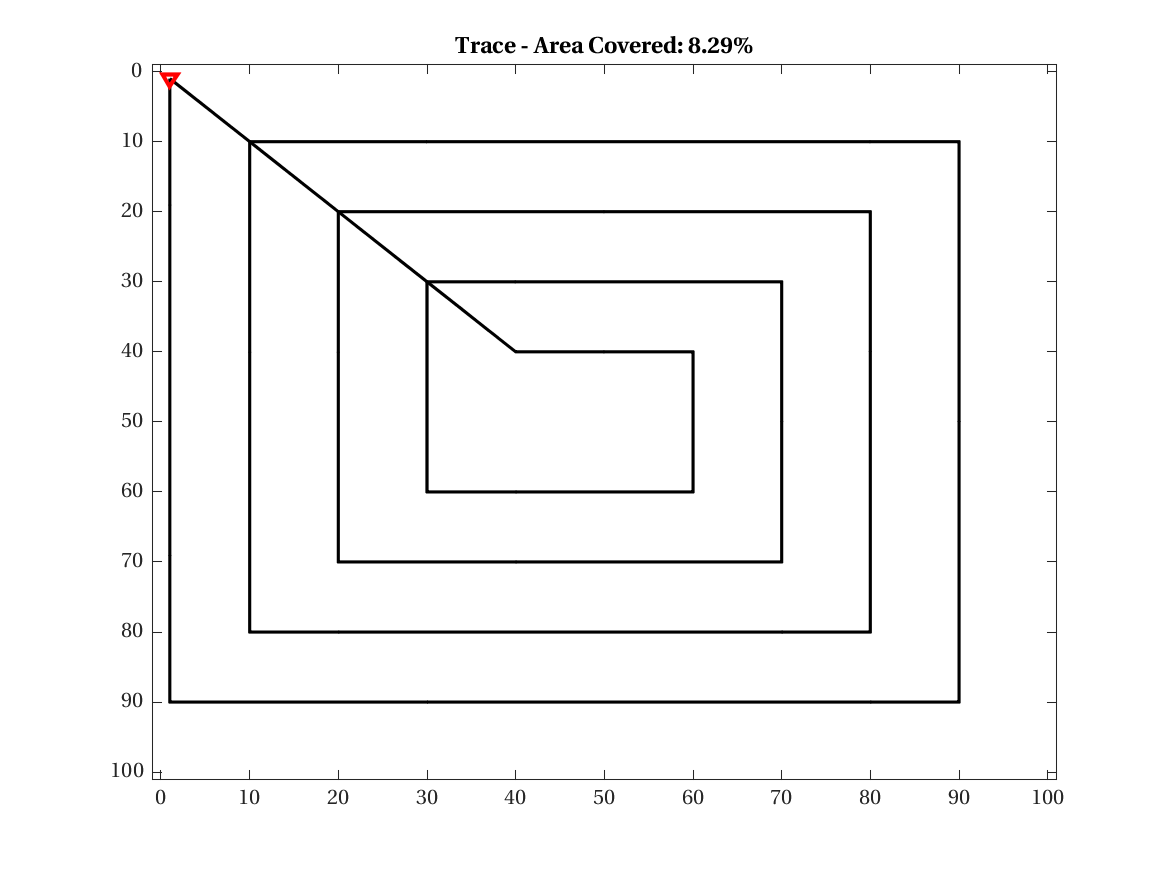
\includegraphics[width=\linewidth]{figures/hbresults/path_zz_10p_100x100_sf_100_seed_2.png}
        \ssp
        \captionsetup{skip=0.20\baselineskip,size=footnotesize}
        \caption{$ZZ_{10}$}
    \end{subfigure}%
    \begin{subfigure}[t]{0.3333\textwidth}
        \centering
        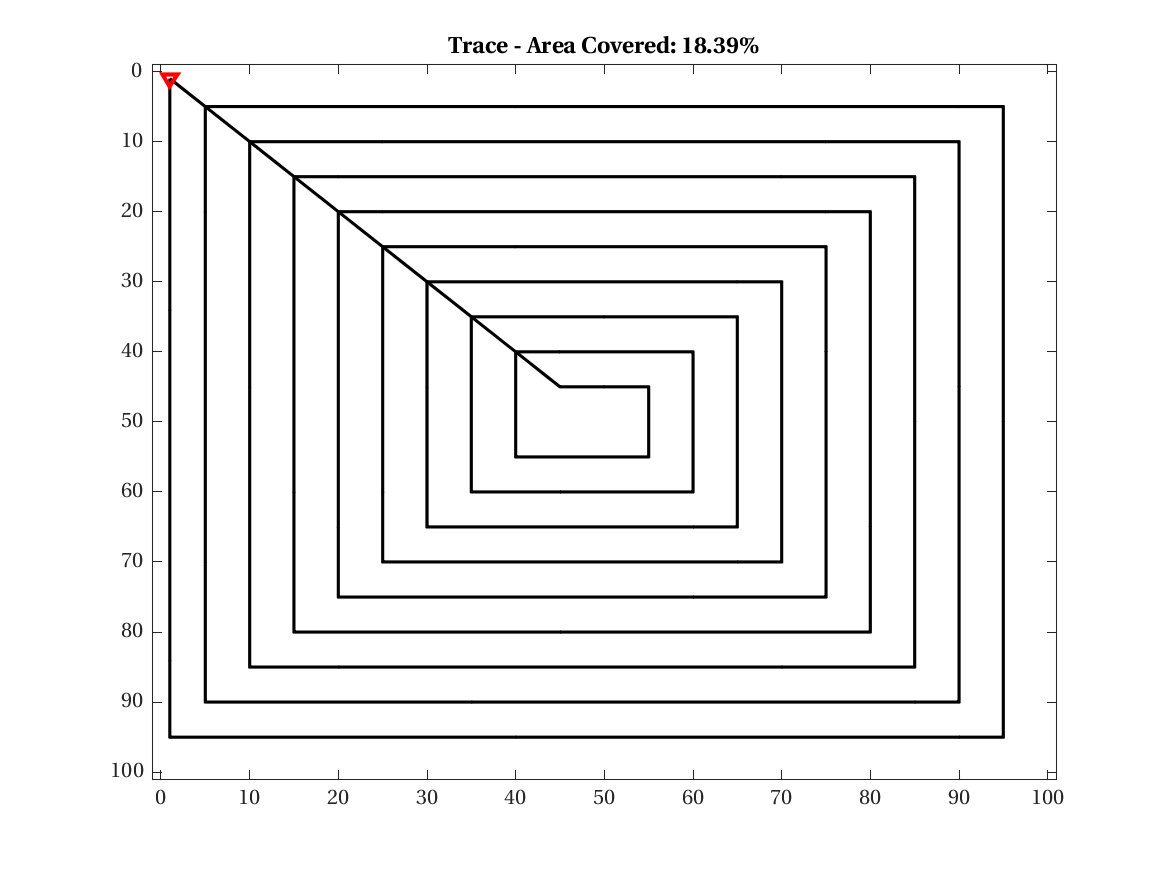
\includegraphics[width=\linewidth]{figures/hbresults/path_zz_20p_100x100_sf_100_seed_2.png}
        \ssp
        \captionsetup{skip=0.20\baselineskip,size=footnotesize}
        \caption{$ZZ_{20}$}
    \end{subfigure}%
    \begin{subfigure}[t]{0.3333\textwidth}
        \centering
        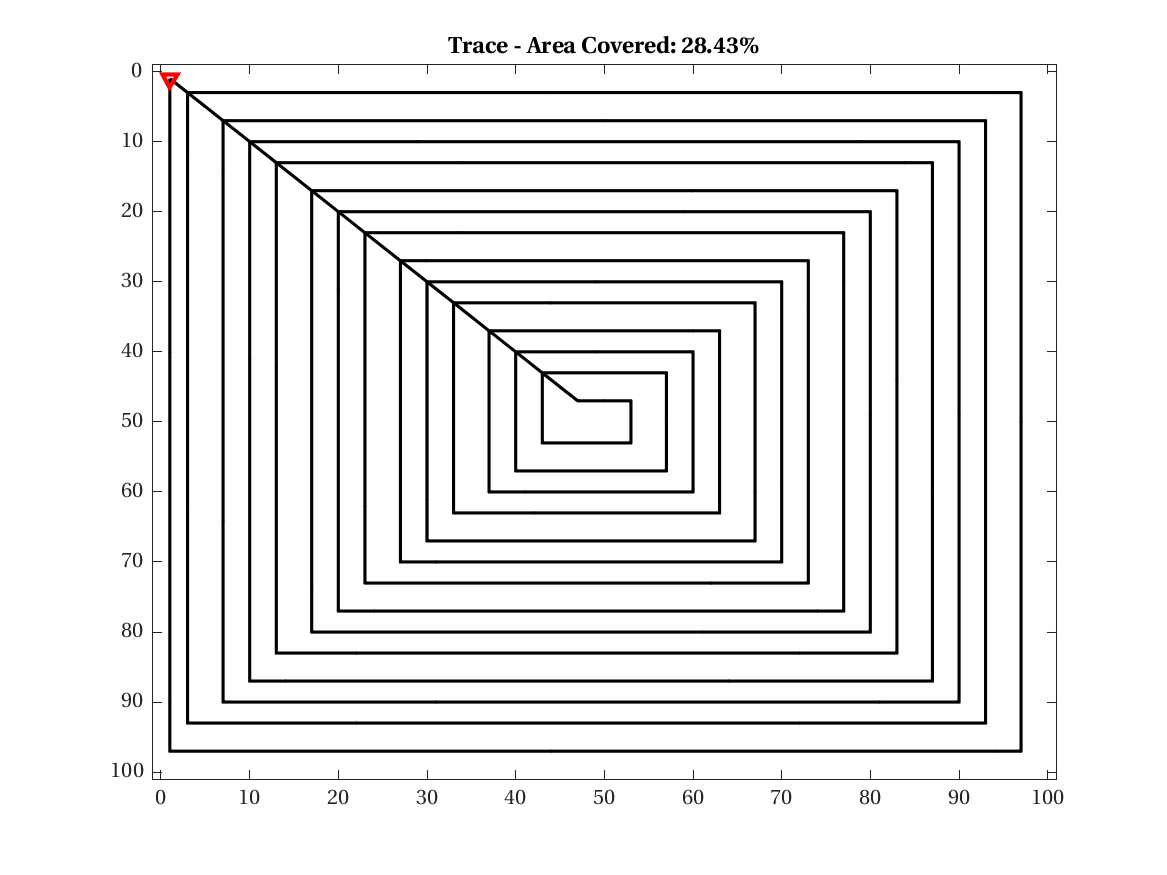
\includegraphics[width=\linewidth]{figures/hbresults/path_zz_30p_100x100_sf_100_seed_2.png}
        \ssp
        \captionsetup{skip=0.20\baselineskip,size=footnotesize}
        \caption{$ZZ_{30}$}
    \end{subfigure}%
    \ssp
    \captionsetup{skip=0.20\baselineskip}
    \caption{Exploration of a field of size $100 \times 100$ using the zig-zag method for three different percentage scan limits.}
    \label{fig:zz102030}
\end{figure}

\section{Prediction Error Calculation}
The quality of each path planner will be judged by its ability to explore a field with a fixed exploration path length. The prediction error of each method will be used as a criterion of path planning quality.

The prediction error function, $E (Z,\hat{Z})$, will be the average root mean square (RMS) error for all $h \times w$ points on the actual field, $Z$, and the predicted field, $\hat{Z}$.

\begin{equation}
E (Z, \hat{Z}) = \frac{1}{hw}\sum_{\forall \vect{s}_i \in Z} (Z(\vect{s}_i) - \hat{Z}(\vect{s}_i))^2
\end{equation}

\section{Comparing to Greedy Next-Best-View}
A course field of size $20 \times 20$ vesicles was generated with a autocorrelation factor, $\sigma_{field}$, equal to $4$, and limited to a $30\%$ scan.

\begin{figure}[htb!]
    \centering
    \begin{subfigure}[t]{0.3333\textwidth}
        \centering
        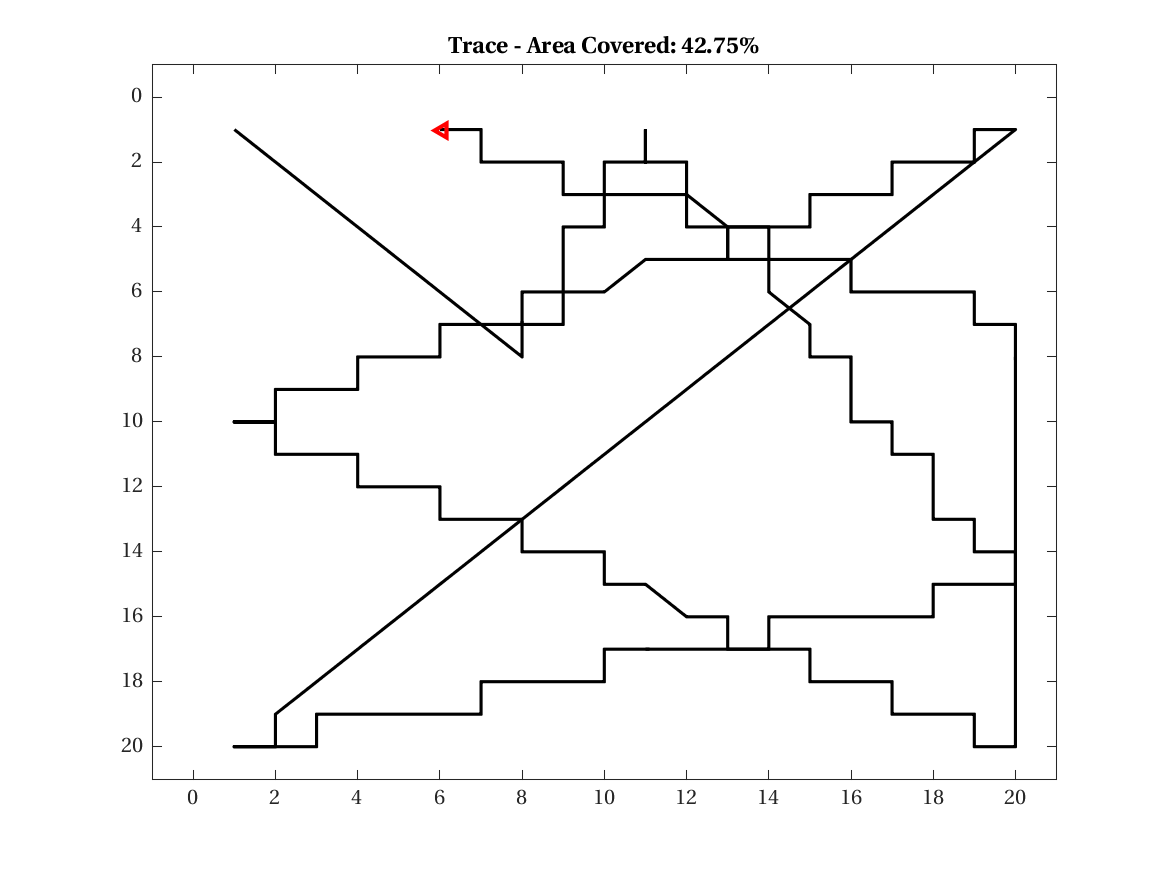
\includegraphics[width=\linewidth]{figures/hbresults/path_nhv_40p_20x20_sf_4_seed_2.png}
        \captionsetup{skip=0.20\baselineskip,size=footnotesize}
        \caption{Highest Variance}
    \end{subfigure}%
    \begin{subfigure}[t]{0.3333\textwidth}
        \centering
        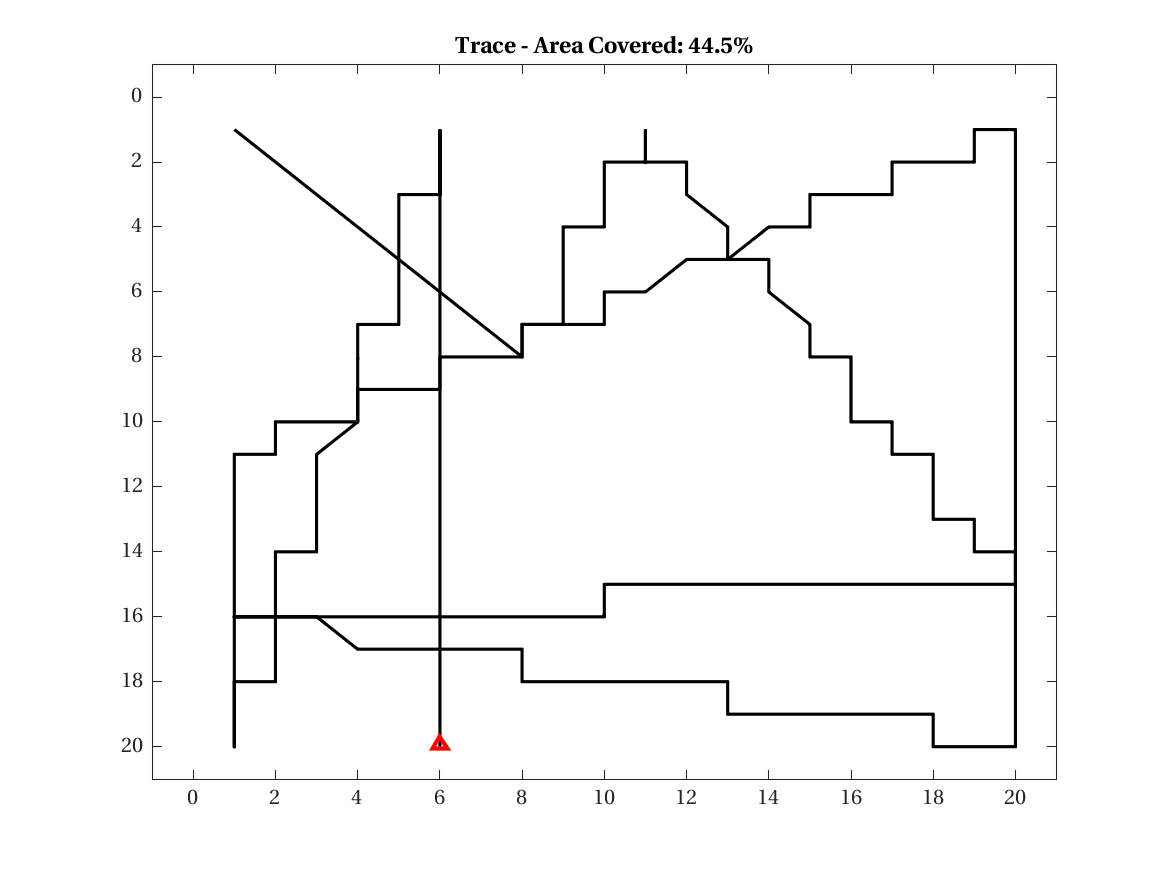
\includegraphics[width=\linewidth]{figures/hbresults/path_nnhv_40p_20x20_sf_4_seed_2.png}
        \captionsetup{skip=0.20\baselineskip,size=footnotesize}
        \caption{$N$ Highest Variance}
    \end{subfigure}%
    \begin{subfigure}[t]{0.3333\textwidth}
        \centering
        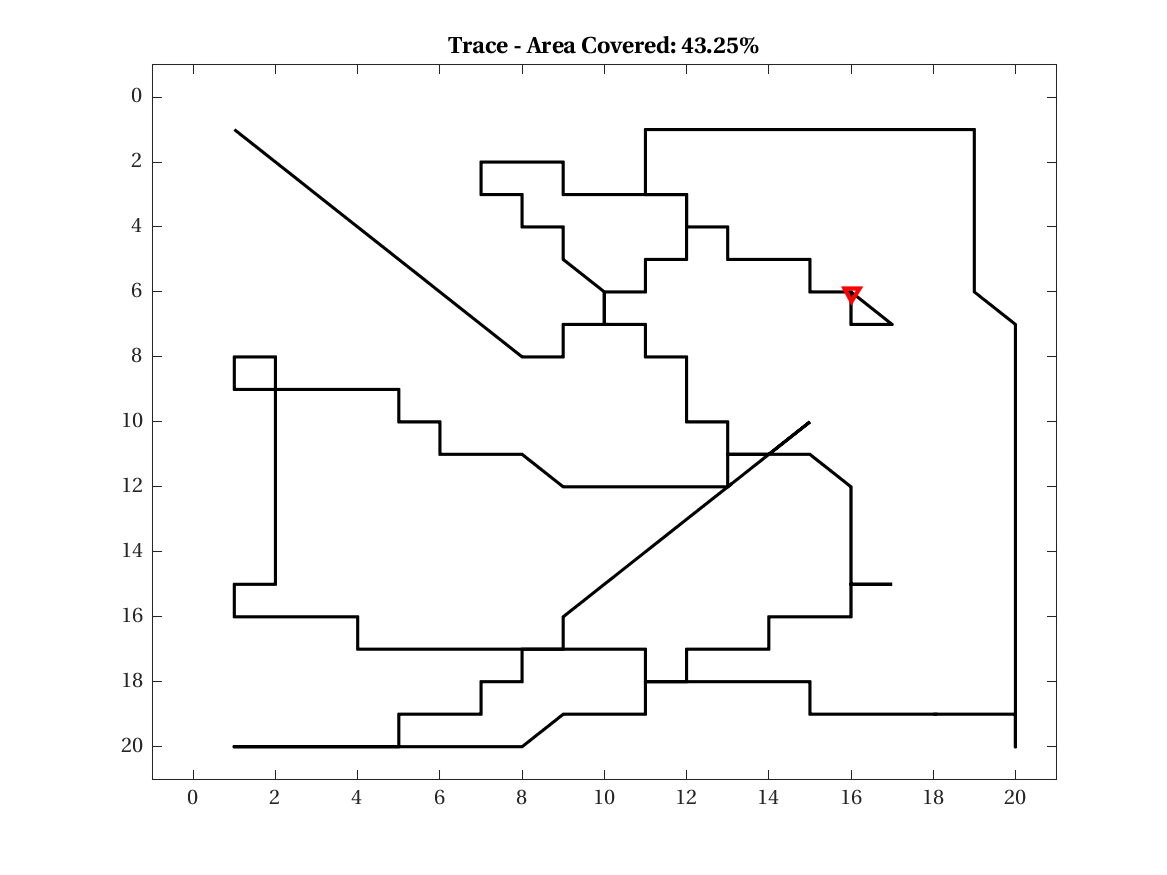
\includegraphics[width=\linewidth]{figures/hbresults/path_mc_40p_20x20_sf_4_seed_2.png}
        \captionsetup{skip=0.20\baselineskip,size=footnotesize}
        \caption{Monte Carlo}
    \end{subfigure}%
    \\
    \begin{subfigure}[t]{0.3333\textwidth}
        \centering
        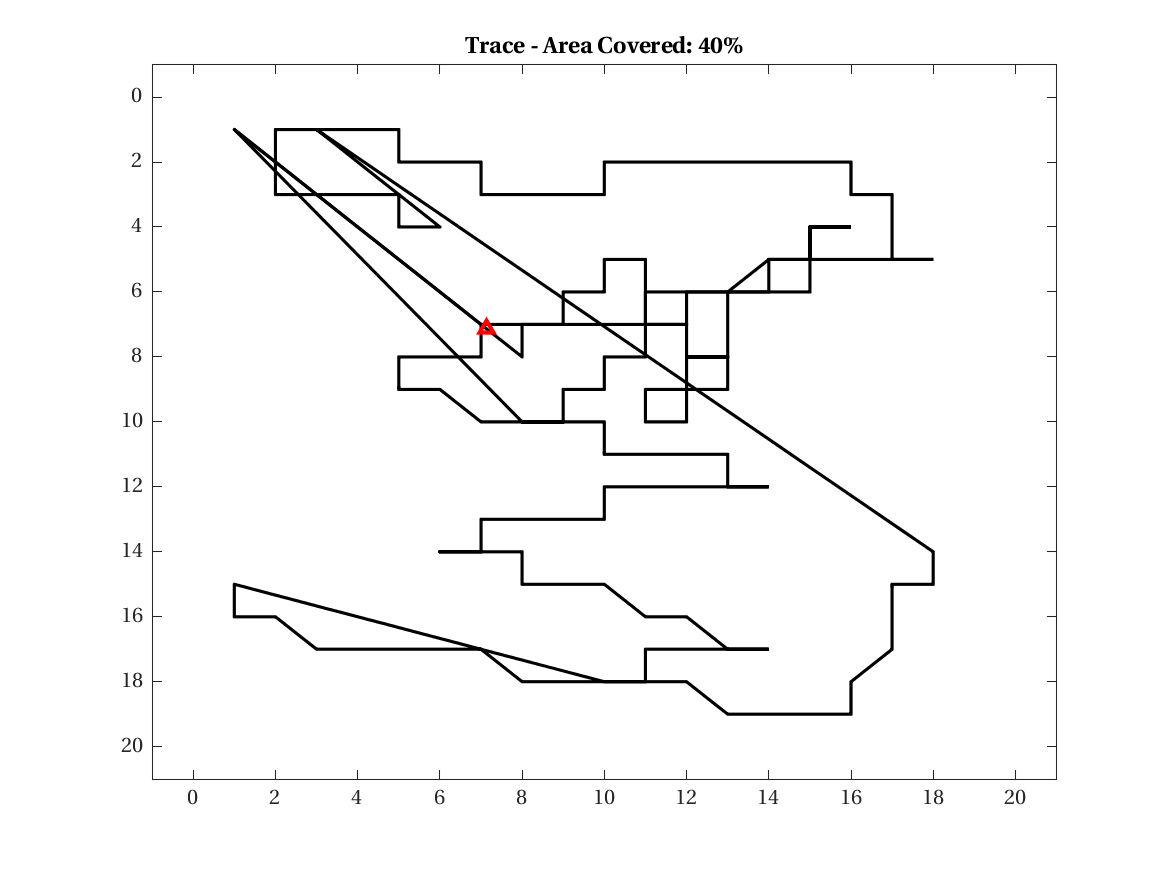
\includegraphics[width=\linewidth]{figures/hbresults/path_nbv_40p_20x20_sf_4_seed_2.png}
        \captionsetup{skip=0.20\baselineskip,size=footnotesize}
        \caption{Greedy NBV}
    \end{subfigure}%
    \begin{subfigure}[t]{0.3333\textwidth}
        \centering
        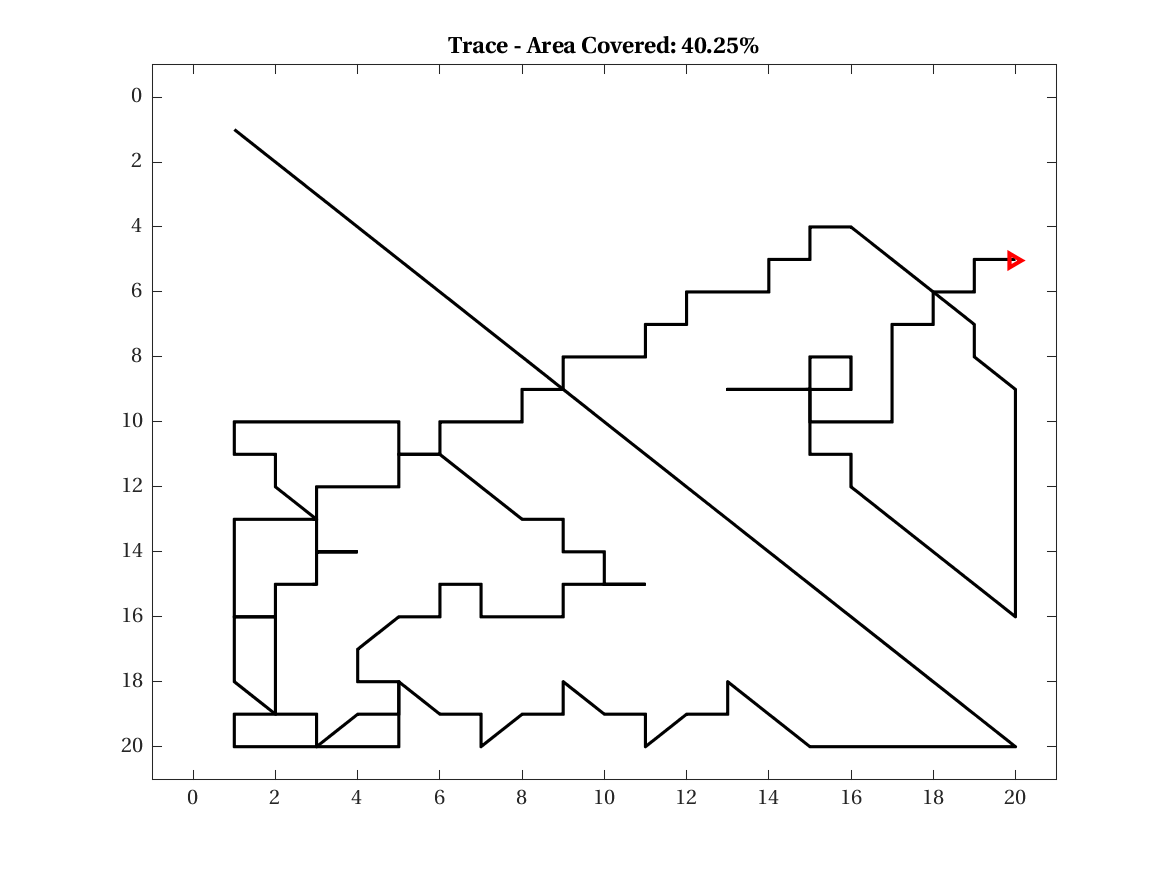
\includegraphics[width=\linewidth]{figures/hbresults/path_gradient_40p_20x20_sf_4_seed_2.png}
        \captionsetup{skip=0.20\baselineskip,size=footnotesize}
        \caption{Gradient Ascent}
    \end{subfigure}%
    \begin{subfigure}[t]{0.3333\textwidth}
        \centering
        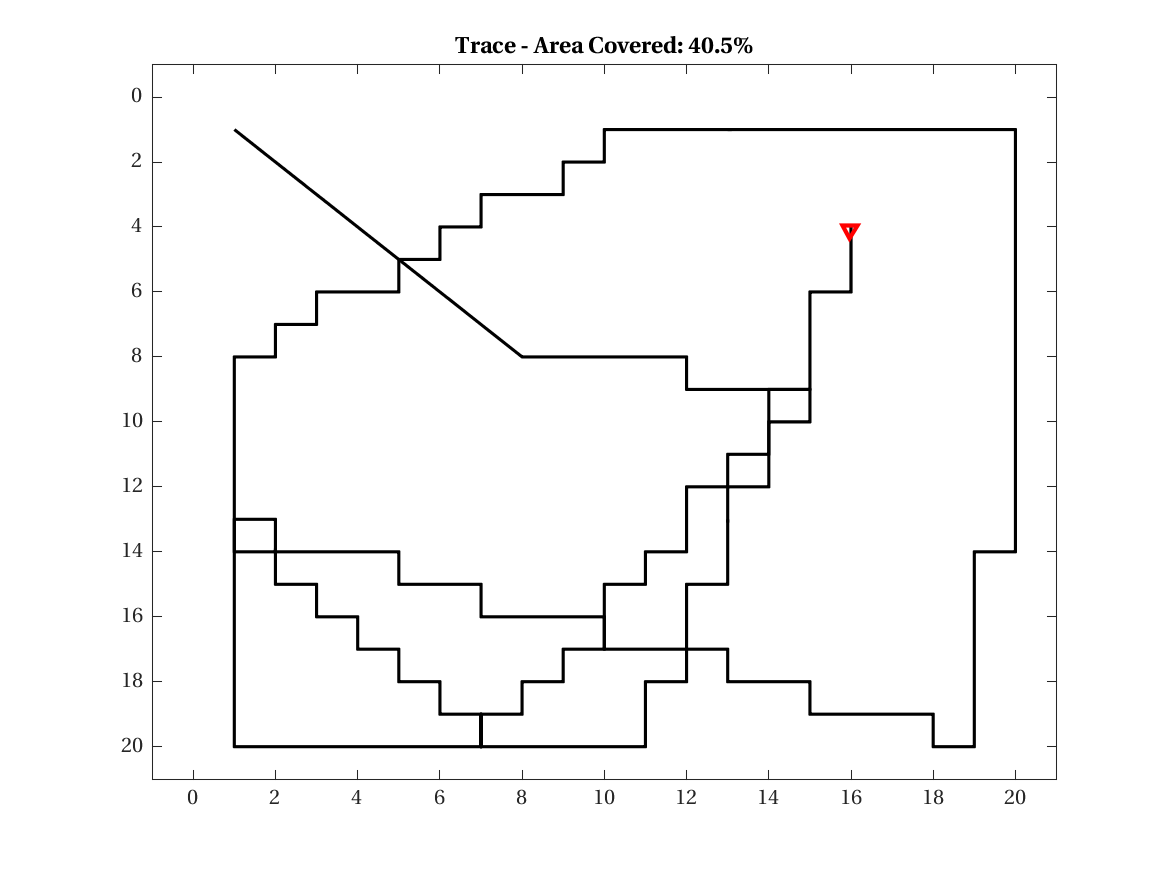
\includegraphics[width=\linewidth]{figures/hbresults/path_gr_40p_20x20_sf_4_seed_2.png}
        \captionsetup{skip=0.20\baselineskip,size=footnotesize}
        \caption{Gradient Range Ascent}
    \end{subfigure}%
    \\
    \begin{subfigure}[t]{0.3333\textwidth}
        \centering
        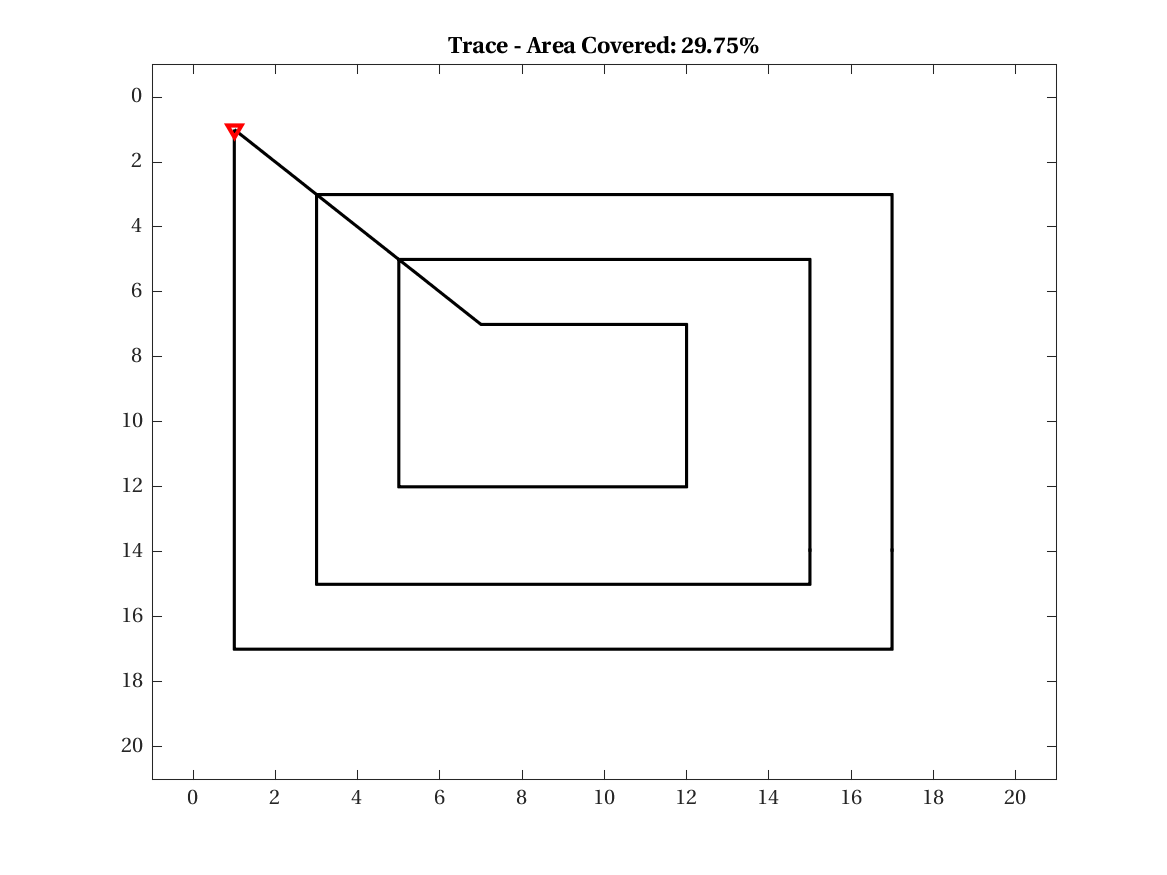
\includegraphics[width=\linewidth]{figures/hbresults/path_zz_40p_20x20_sf_4_seed_2.png}
        \captionsetup{skip=0.20\baselineskip,size=footnotesize}
        \caption{$ZZ_{30}$}
    \end{subfigure}%
    \captionsetup{skip=0.20\baselineskip}
    \caption{Exploration of a field of size $20 \times 20$, $\sigma_{field} = 4$, random seed 2.}
    \label{fig:nbvpathcomp}
\end{figure}

\begin{figure}[htb!]
    \centering
    \begin{subfigure}[t]{0.75\textwidth}
        \centering
        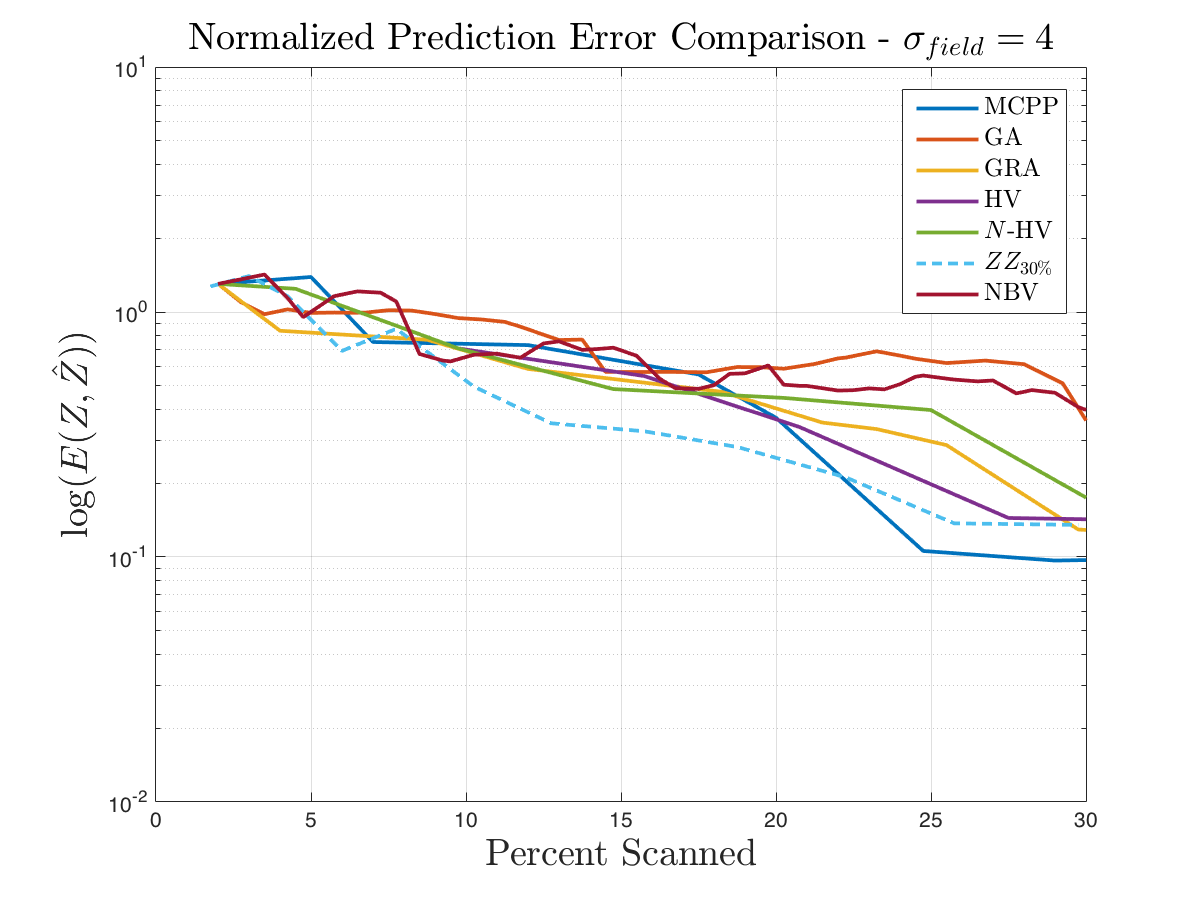
\includegraphics[width=\linewidth]{figures/results/normalized_errors_40p_20x20_sf_4_seed_2_app_10.png}
        \captionsetup{skip=0.20\baselineskip,size=footnotesize}
        \caption{Normalized prediction errors for each method.}
    \end{subfigure}%
    \\
    \begin{subfigure}[t]{0.75\textwidth}
        \centering
        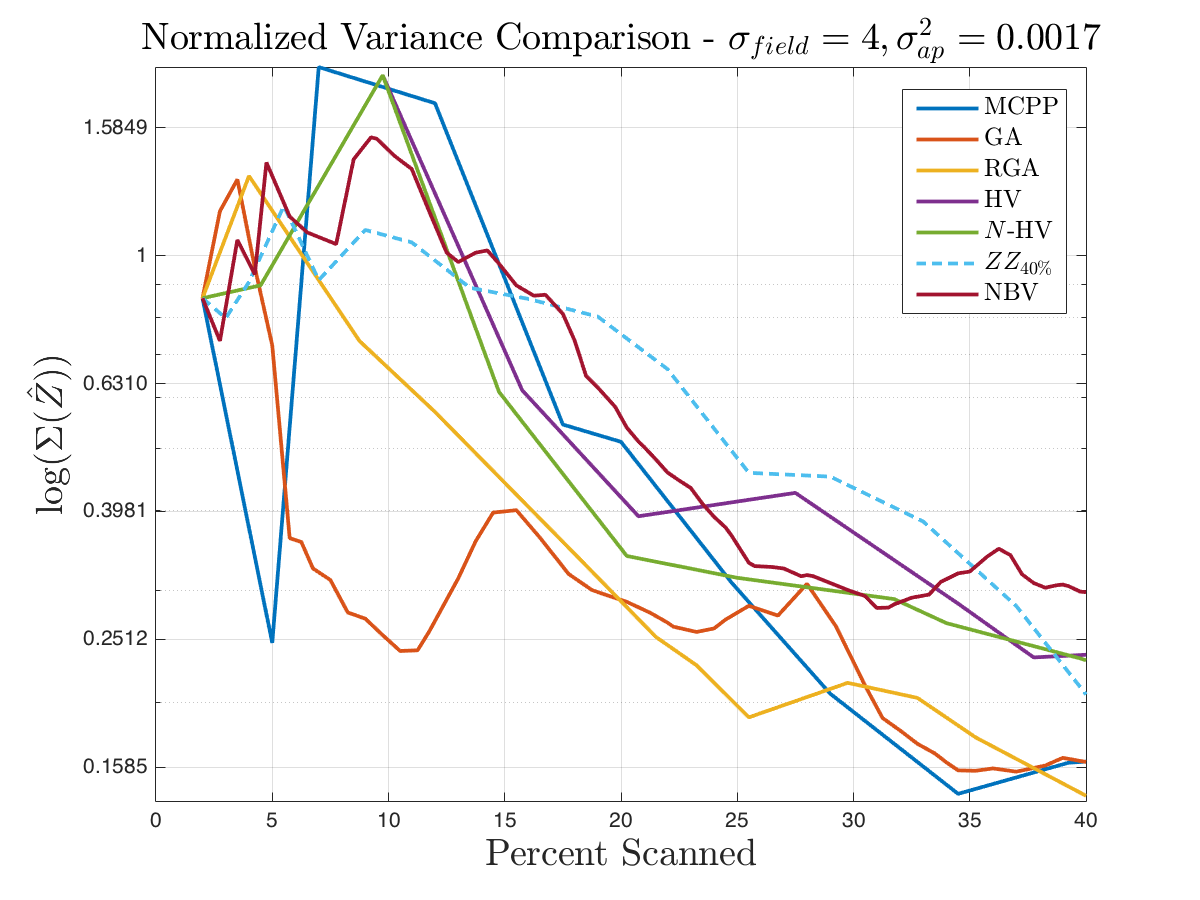
\includegraphics[width=\linewidth]{figures/results/normalized_variances_40p_20x20_sf_4_seed_2_app_10.png}
        \captionsetup{skip=0.20\baselineskip,size=footnotesize}
        \caption{Normalized prediction variances for each method.}
    \end{subfigure}%
    \captionsetup{skip=0.20\baselineskip}
    \caption{Prediction error and variances for an exploration of a field of size $20 \times 20$, $\sigma_{field} = 4$, random seed 2.}
    \label{fig:nbvcomp}
\end{figure}

\FloatBarrier
\clearpage

\section{High Spatial Autocorrelation Results}
The methods will be compared on target fields generated with an autocorrelation factor, $\sigma_{field}$, equal to the field width. A Gaussian filter $G(x,y,100)$ (Equation \ref{eq:gauss_filt}), is convolved with all points on the field.

\begin{figure}[htb!]
    \centering
    \begin{subfigure}[t]{0.3333\textwidth}
        \centering
        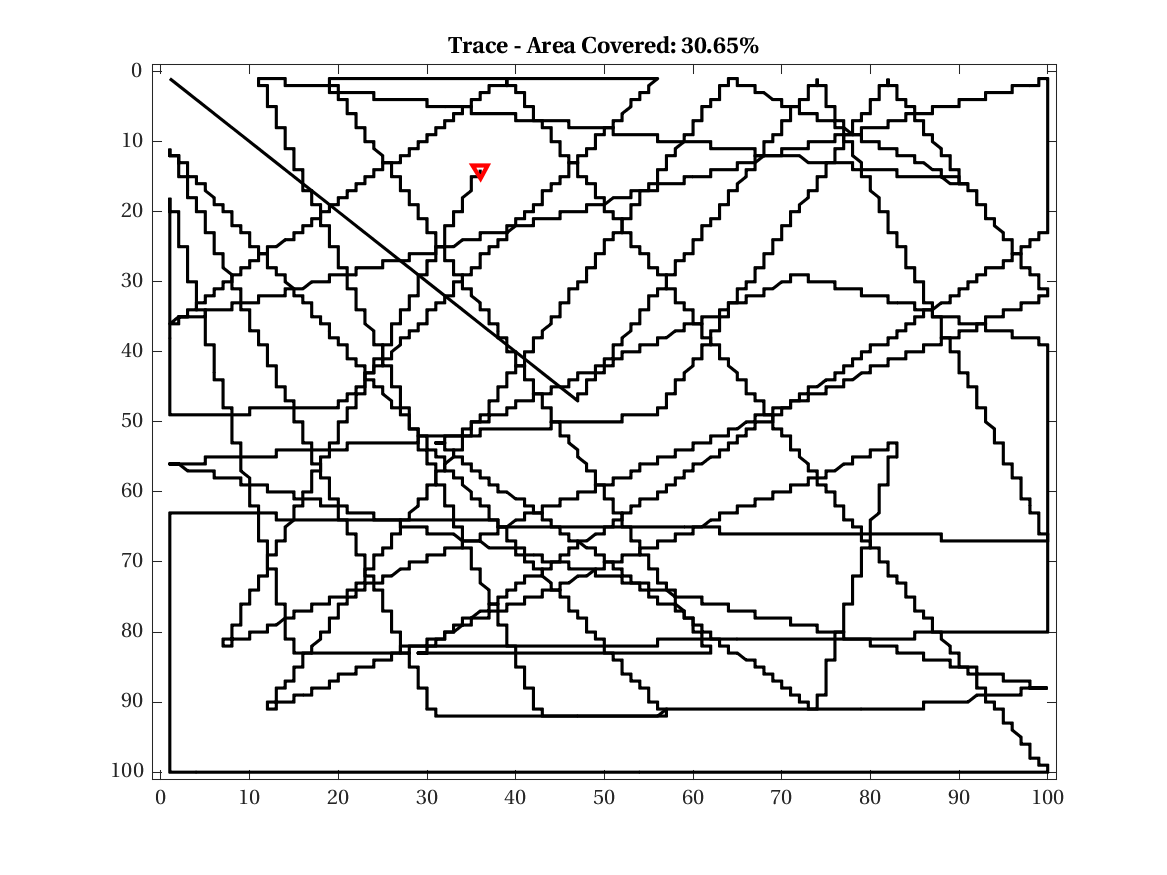
\includegraphics[width=\linewidth]{figures/hbresults/path_nhv_30p_100x100_sf_100_seed_2.png}
        \captionsetup{skip=0.20\baselineskip,size=footnotesize}
        \caption{Highest Variance}
    \end{subfigure}%
    \begin{subfigure}[t]{0.3333\textwidth}
        \centering
        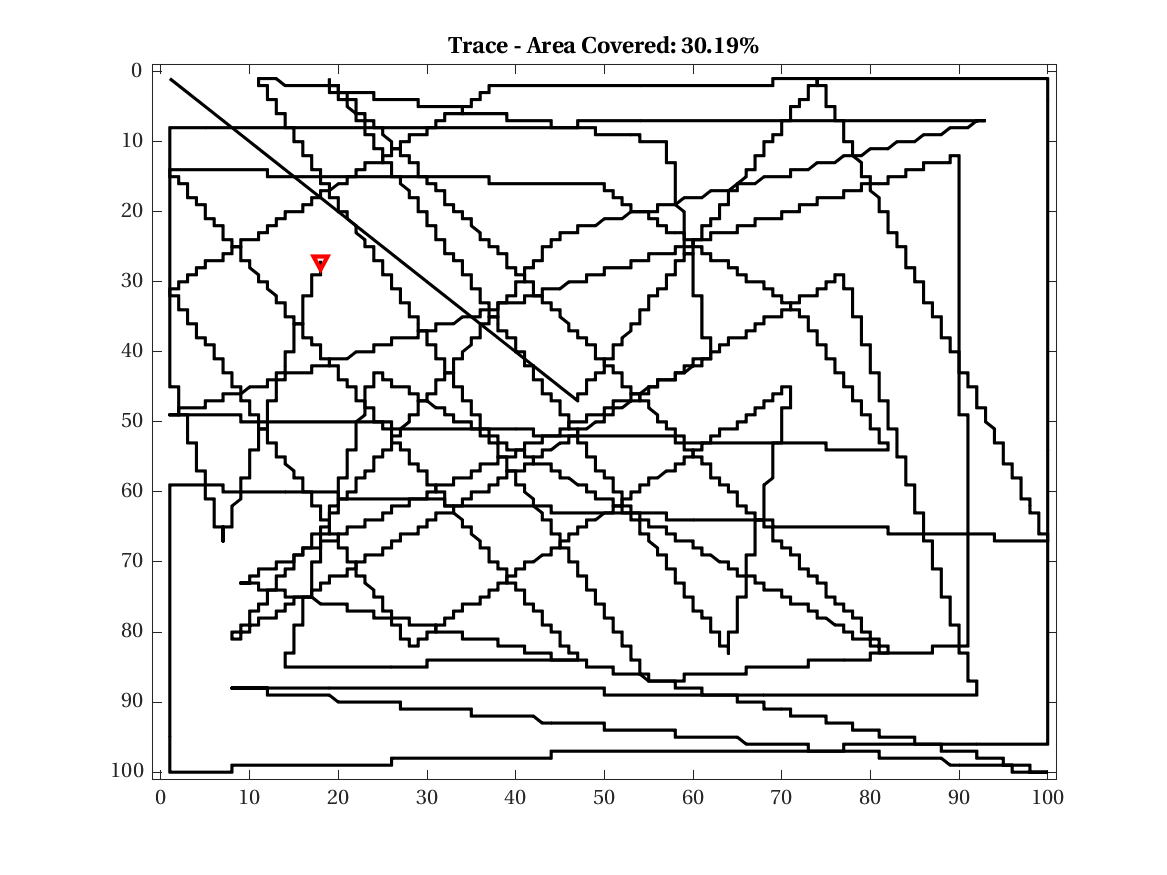
\includegraphics[width=\linewidth]{figures/hbresults/path_nnhv_30p_100x100_sf_100_seed_2.png}
        \captionsetup{skip=0.20\baselineskip,size=footnotesize}
        \caption{$N$ Highest Variance}
    \end{subfigure}%
    \begin{subfigure}[t]{0.3333\textwidth}
        \centering
        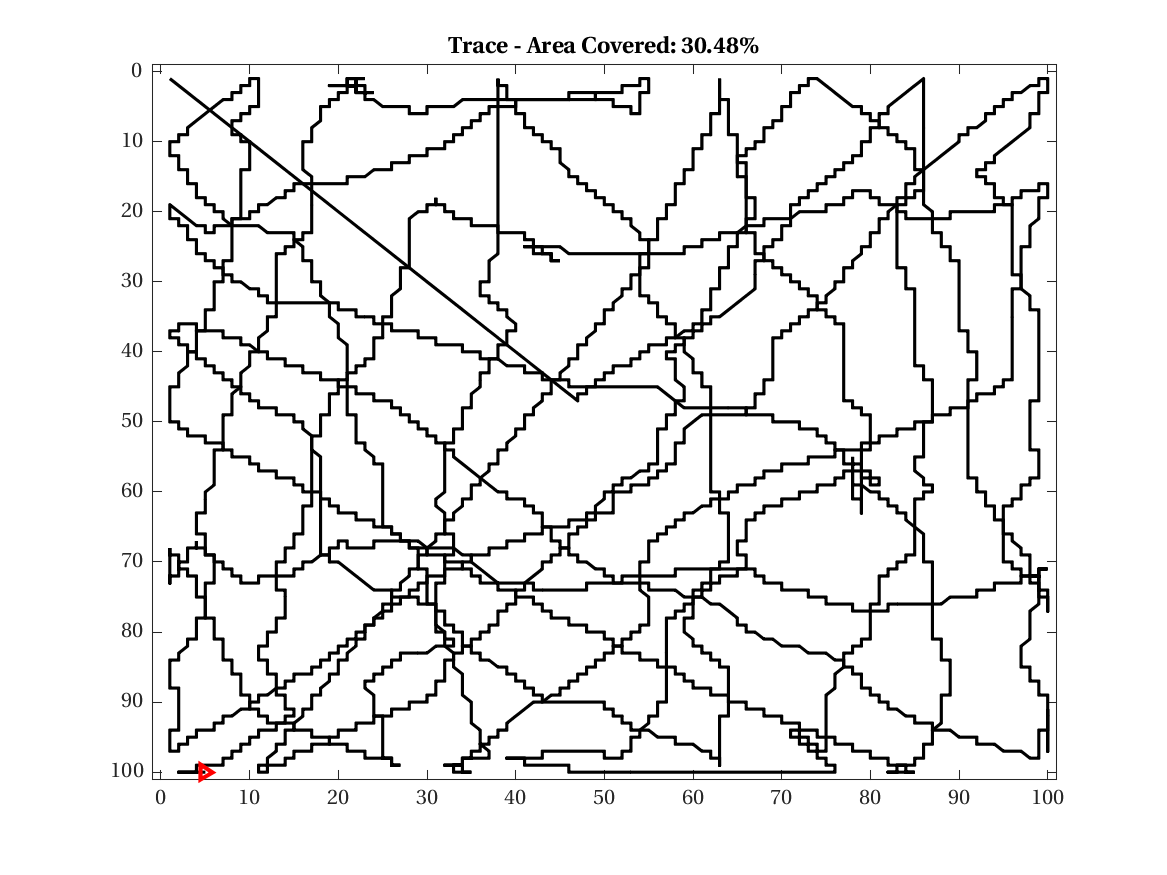
\includegraphics[width=\linewidth]{figures/hbresults/path_mc_30p_100x100_sf_100_seed_2.png}
        \captionsetup{skip=0.20\baselineskip,size=footnotesize}
        \caption{Monte Carlo}
    \end{subfigure}%
    \\
    \begin{subfigure}[t]{0.3333\textwidth}
        \centering
        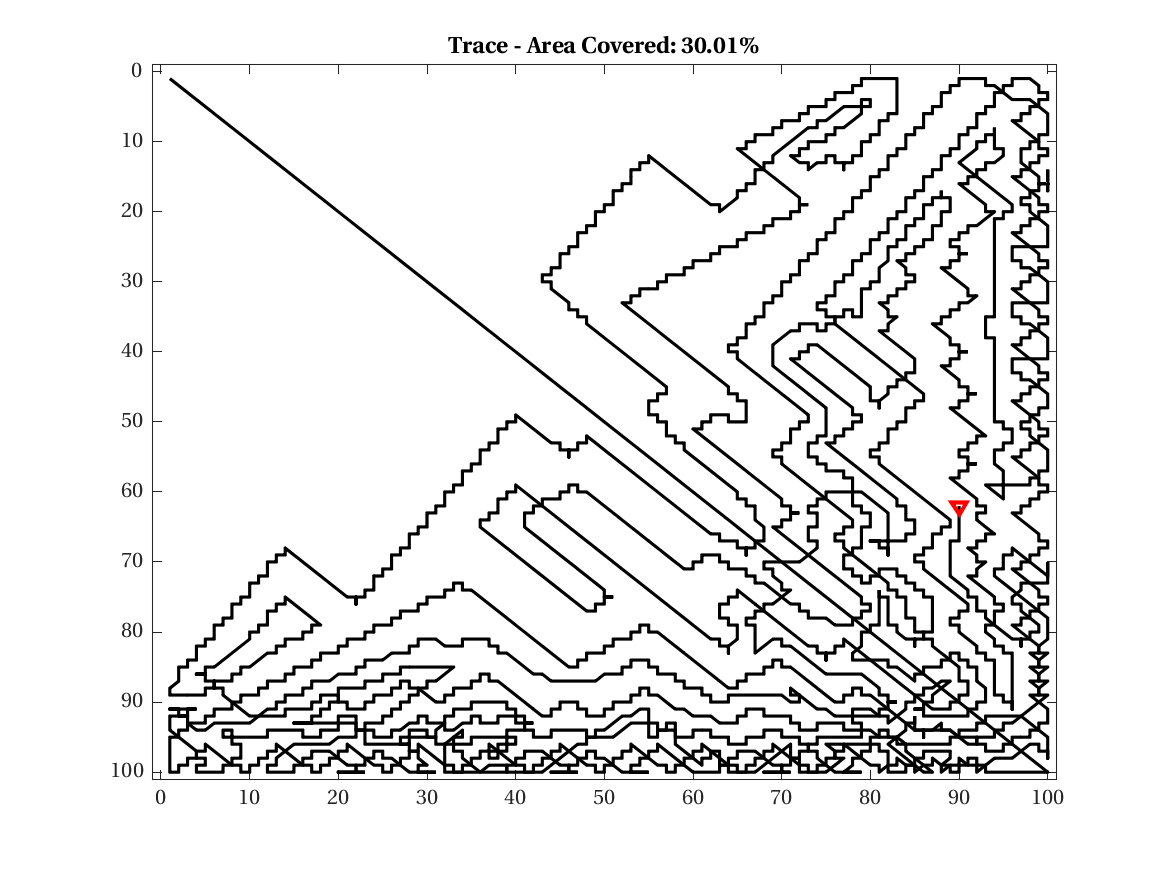
\includegraphics[width=\linewidth]{figures/hbresults/path_gradient_30p_100x100_sf_100_seed_2.png}
        \captionsetup{skip=0.20\baselineskip,size=footnotesize}
        \caption{Gradient Ascent}
    \end{subfigure}%
    \begin{subfigure}[t]{0.3333\textwidth}
        \centering
        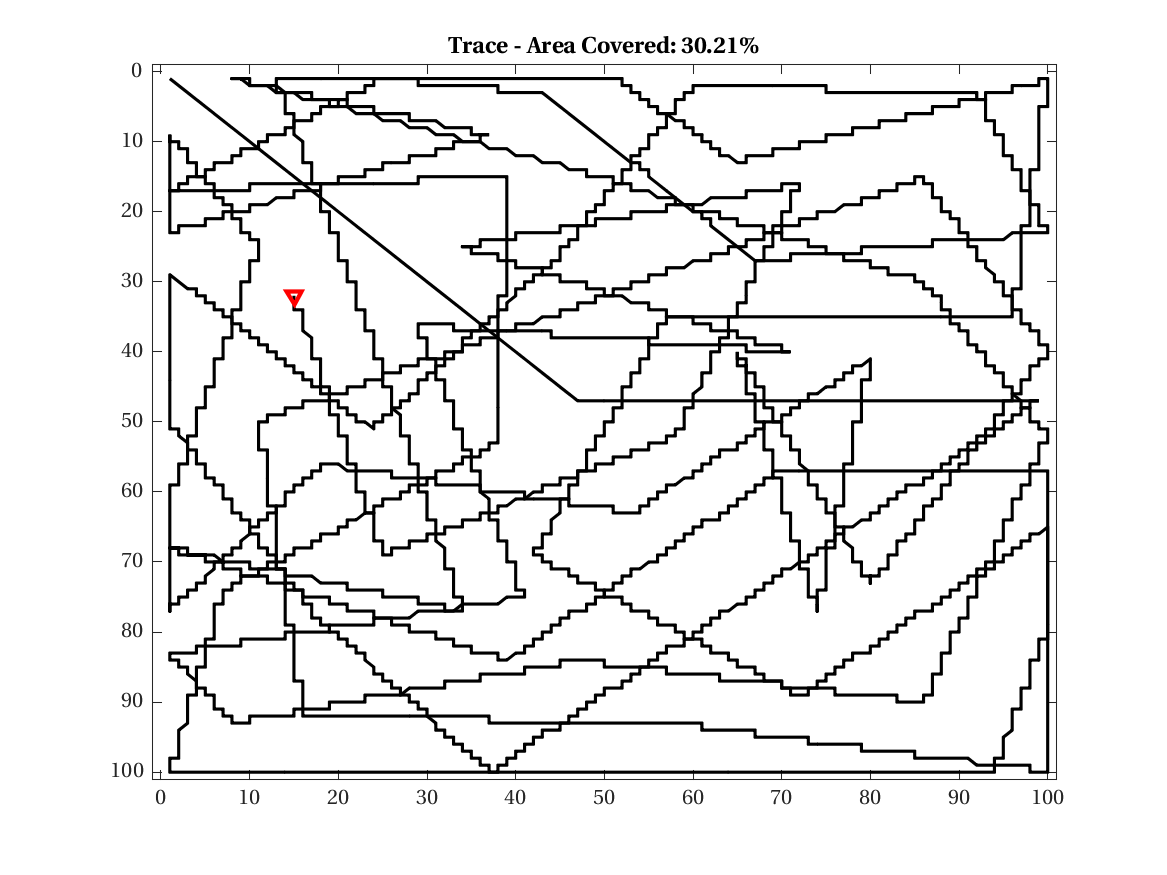
\includegraphics[width=\linewidth]{figures/hbresults/path_gr_30p_100x100_sf_100_seed_2.png}
        \captionsetup{skip=0.20\baselineskip,size=footnotesize}
        \caption{Gradient Range Ascent}
    \end{subfigure}%
    \\
    \begin{subfigure}[t]{0.3333\textwidth}
        \centering
        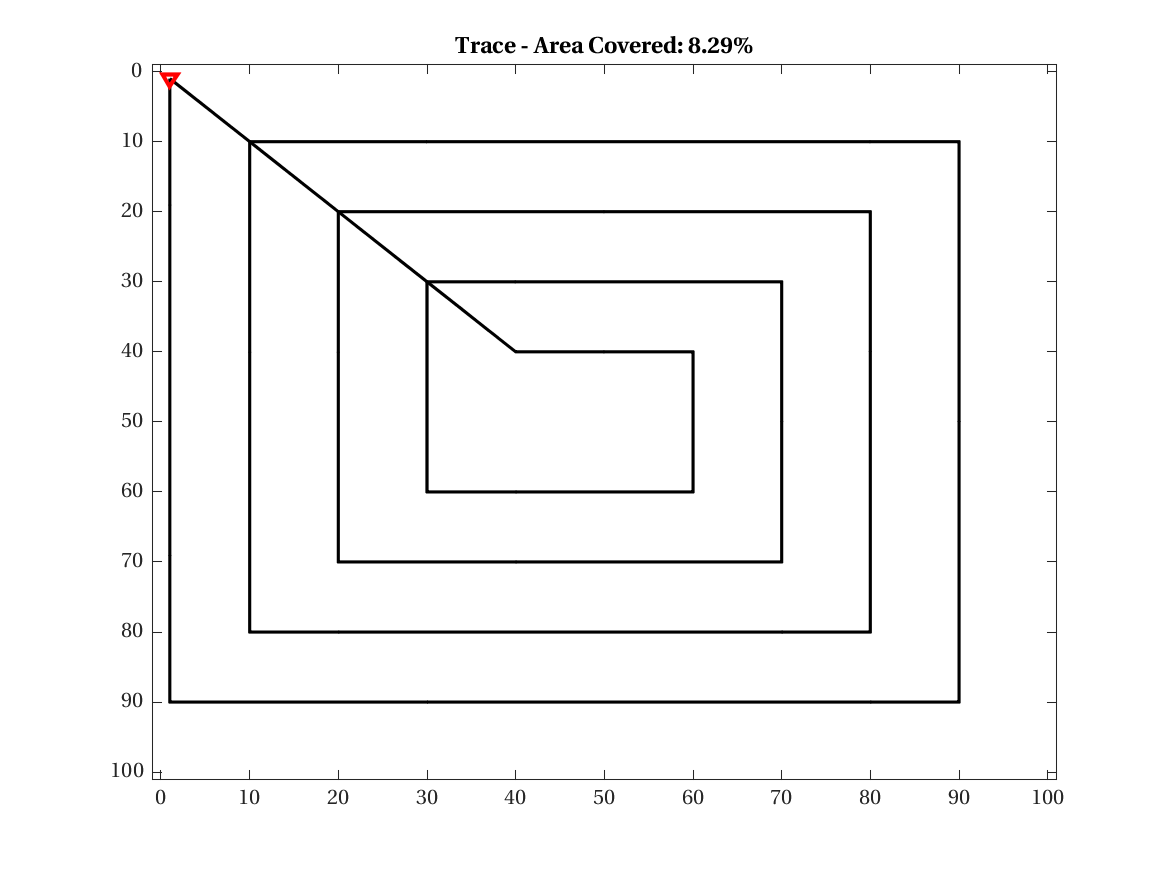
\includegraphics[width=\linewidth]{figures/hbresults/path_zz_10p_100x100_sf_100_seed_2.png}
        \captionsetup{skip=0.20\baselineskip,size=footnotesize}
        \caption{$ZZ_{10}$}
    \end{subfigure}%
    \begin{subfigure}[t]{0.3333\textwidth}
        \centering
        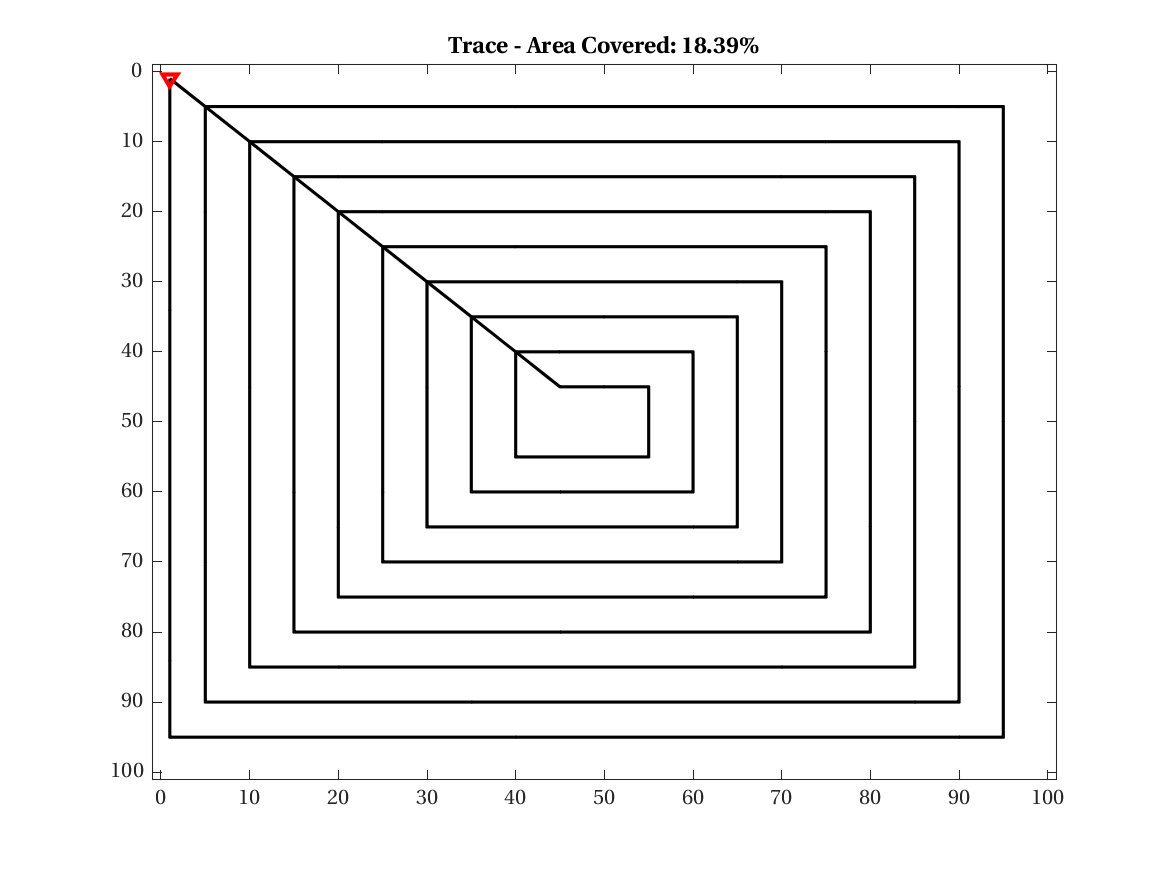
\includegraphics[width=\linewidth]{figures/hbresults/path_zz_20p_100x100_sf_100_seed_2.png}
        \captionsetup{skip=0.20\baselineskip,size=footnotesize}
        \caption{$ZZ_{20}$}
    \end{subfigure}%
    \begin{subfigure}[t]{0.3333\textwidth}
        \centering
        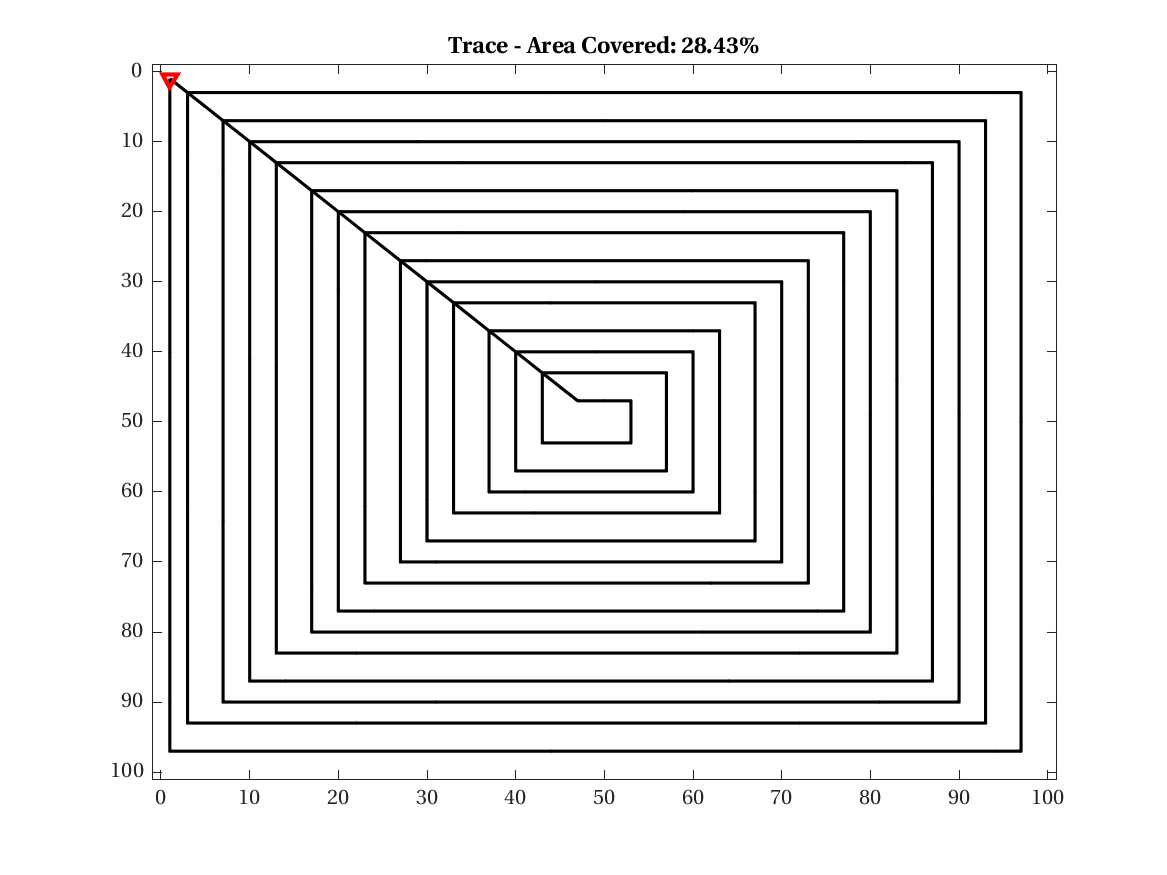
\includegraphics[width=\linewidth]{figures/hbresults/path_zz_30p_100x100_sf_100_seed_2.png}
        \captionsetup{skip=0.20\baselineskip,size=footnotesize}
        \caption{$ZZ_{30}$}
    \end{subfigure}%
    \captionsetup{skip=0.20\baselineskip}
    \caption{Exploration of a field of size $100 \times 100$, $\sigma_{field} = 100$, random seed 2.}
    \label{fig:sf100}
\end{figure}

\begin{figure}[htb!]
    \centering
    \begin{subfigure}[t]{0.75\textwidth}
        \centering
        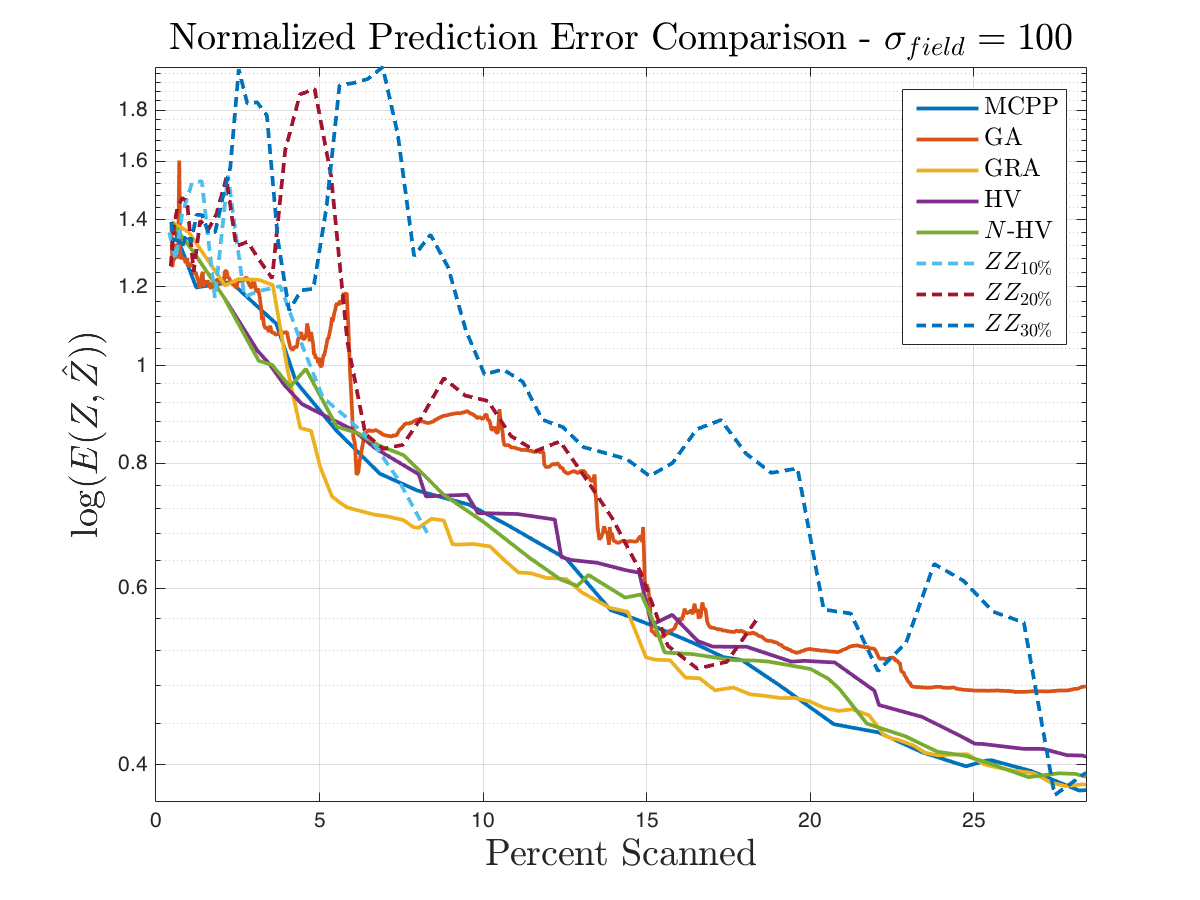
\includegraphics[width=\linewidth]{figures/results/normalized_errors_30p_100x100_sf_100_seed_2_app_50.png}
        \captionsetup{skip=0.20\baselineskip,size=footnotesize}
        \caption{Normalized prediction errors for each method.}
    \end{subfigure}%
    \\
    \begin{subfigure}[t]{0.75\textwidth}
        \centering
        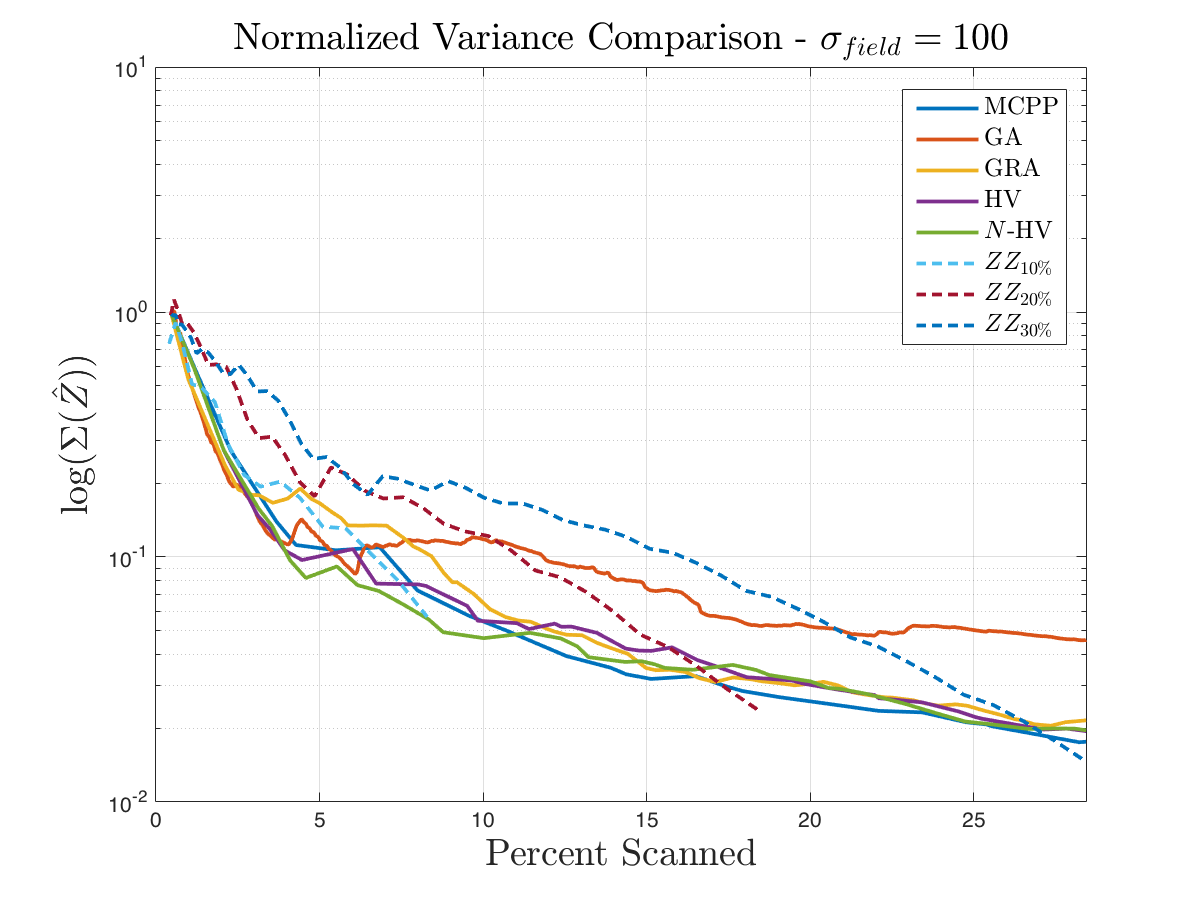
\includegraphics[width=\linewidth]{figures/results/normalized_variances_30p_100x100_sf_100_seed_2_app_50.png}
        \captionsetup{skip=0.20\baselineskip,size=footnotesize}
        \caption{Normalized prediction variances for each method.}
    \end{subfigure}%
    \captionsetup{skip=0.20\baselineskip}
    \caption{Prediction error and variances for an exploration of a field of size $100 \times 100$, $\sigma_{field} = 100$, random seed 2.}
    \label{fig:errvar100}
\end{figure}

\FloatBarrier
\clearpage

\section{Half Width Spatial Autocorrelation Results}
The methods will be compared on target fields generated with an autocorrelation factor, $\sigma_{field}$, equal to the half of the target field's width. A Gaussian filter $G(x,y,50)$ (Equation \ref{eq:gauss_filt}), is convolved with all points on the field.

\begin{figure}[htb!]
    \centering
    \begin{subfigure}[t]{0.3333\textwidth}
        \centering
        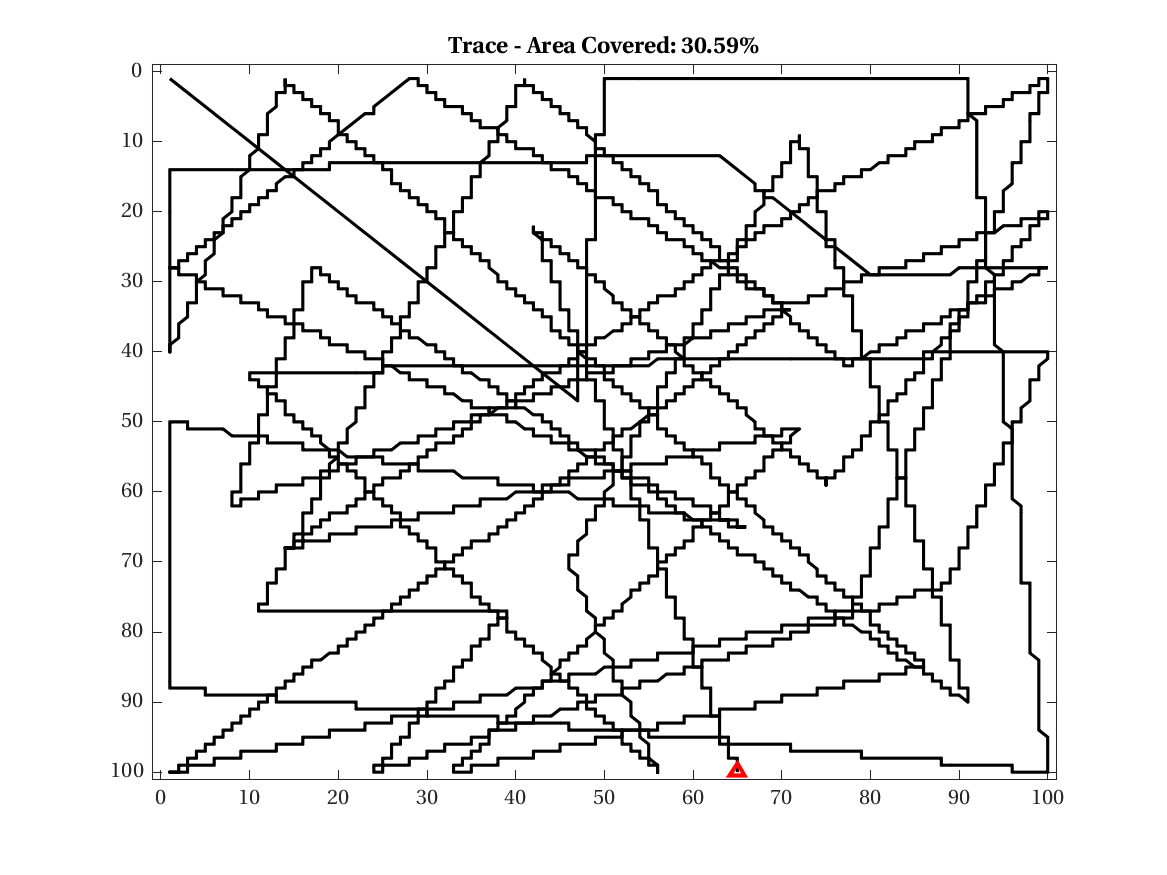
\includegraphics[width=\linewidth]{figures/hbresults/path_nhv_30p_100x100_sf_50_seed_2.png}
        \captionsetup{skip=0.20\baselineskip,size=footnotesize}
        \caption{Highest Variance}
    \end{subfigure}%
    \begin{subfigure}[t]{0.3333\textwidth}
        \centering
        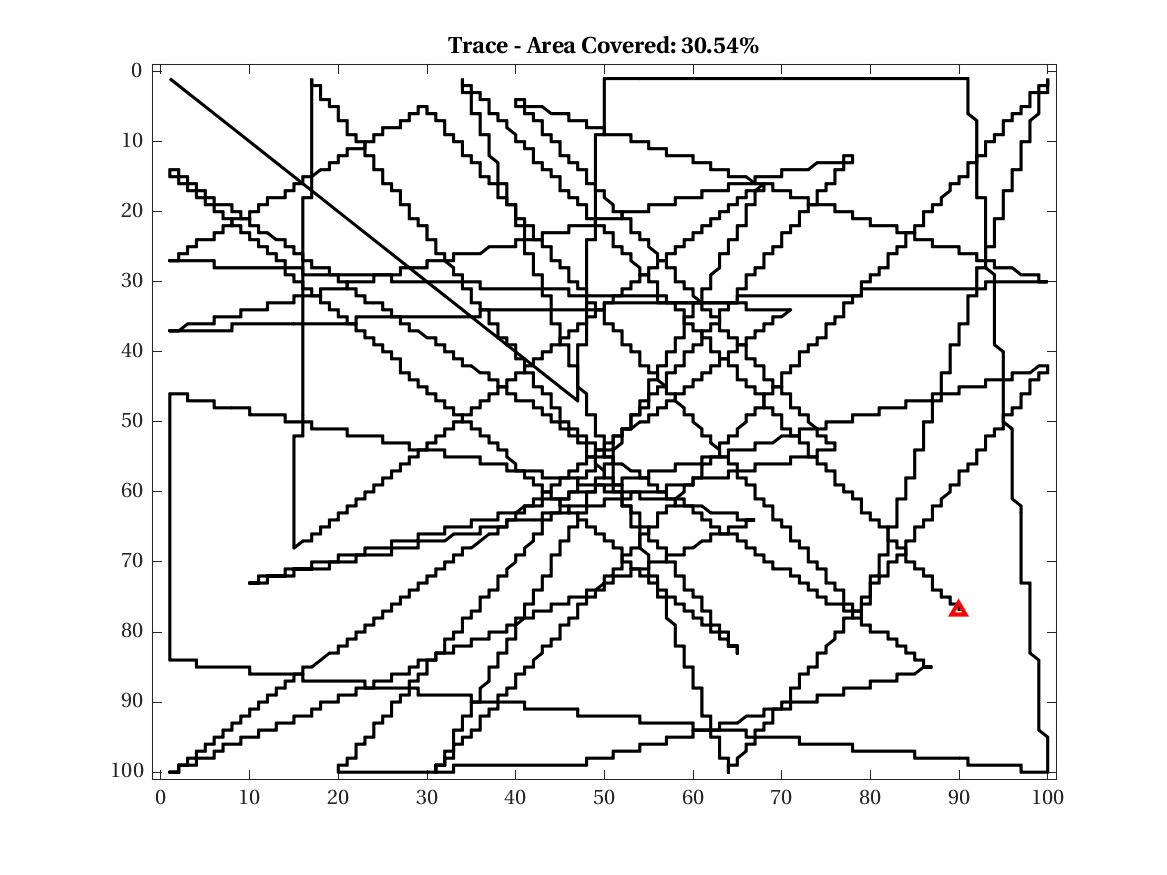
\includegraphics[width=\linewidth]{figures/hbresults/path_nnhv_30p_100x100_sf_50_seed_2.png}
        \captionsetup{skip=0.20\baselineskip,size=footnotesize}
        \caption{$N$ Highest Variance}
    \end{subfigure}%
    \begin{subfigure}[t]{0.3333\textwidth}
        \centering
        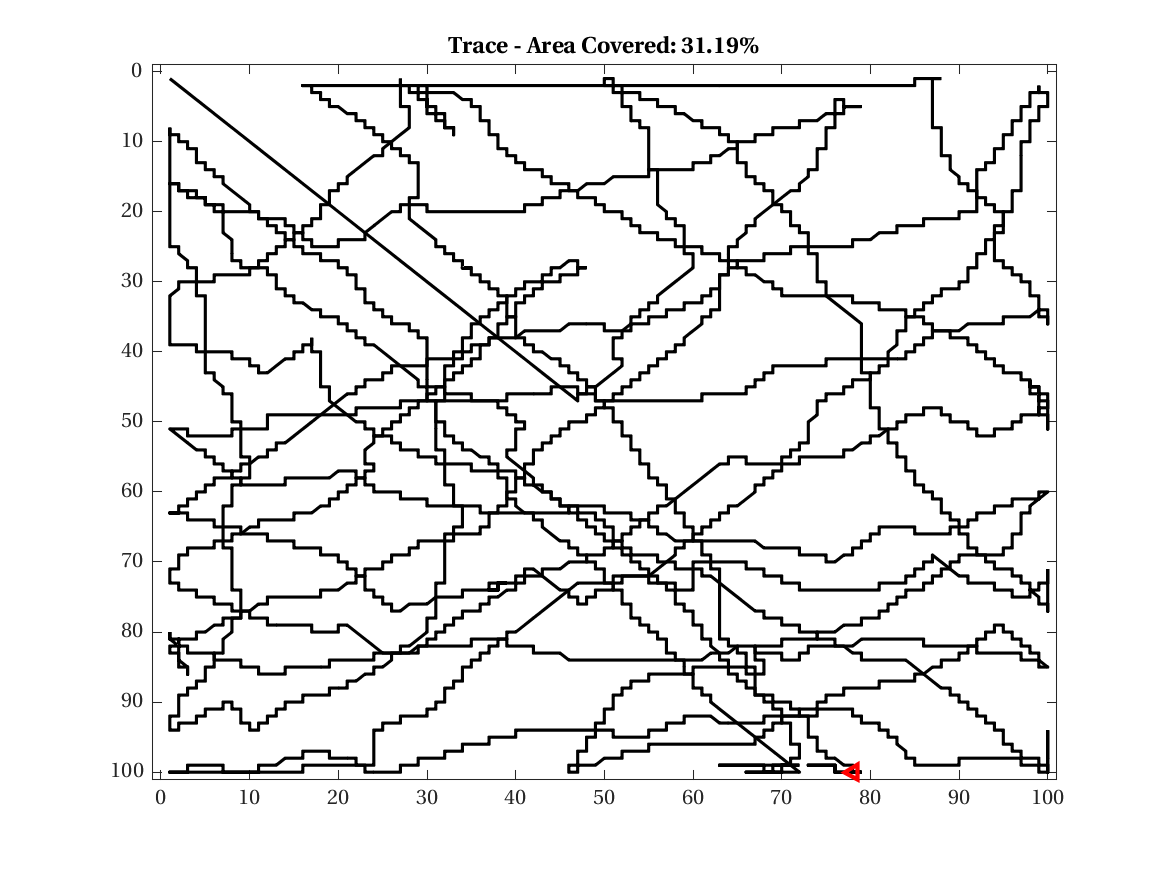
\includegraphics[width=\linewidth]{figures/hbresults/path_mc_30p_100x100_sf_50_seed_2.png}
        \captionsetup{skip=0.20\baselineskip,size=footnotesize}
        \caption{Monte Carlo}
    \end{subfigure}%
    \\
    \begin{subfigure}[t]{0.3333\textwidth}
        \centering
        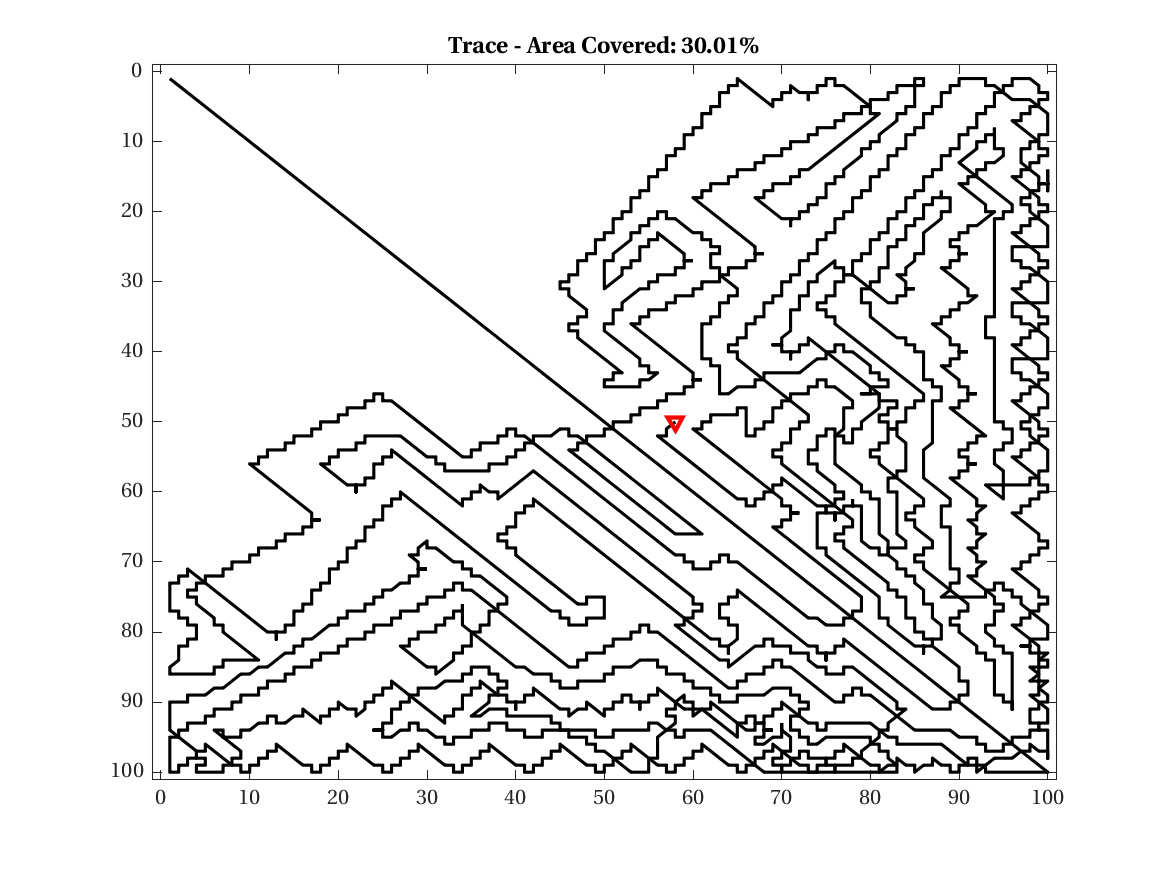
\includegraphics[width=\linewidth]{figures/hbresults/path_gradient_30p_100x100_sf_50_seed_2.png}
        \captionsetup{skip=0.20\baselineskip,size=footnotesize}
        \caption{Gradient Ascent}
    \end{subfigure}%
    \begin{subfigure}[t]{0.3333\textwidth}
        \centering
        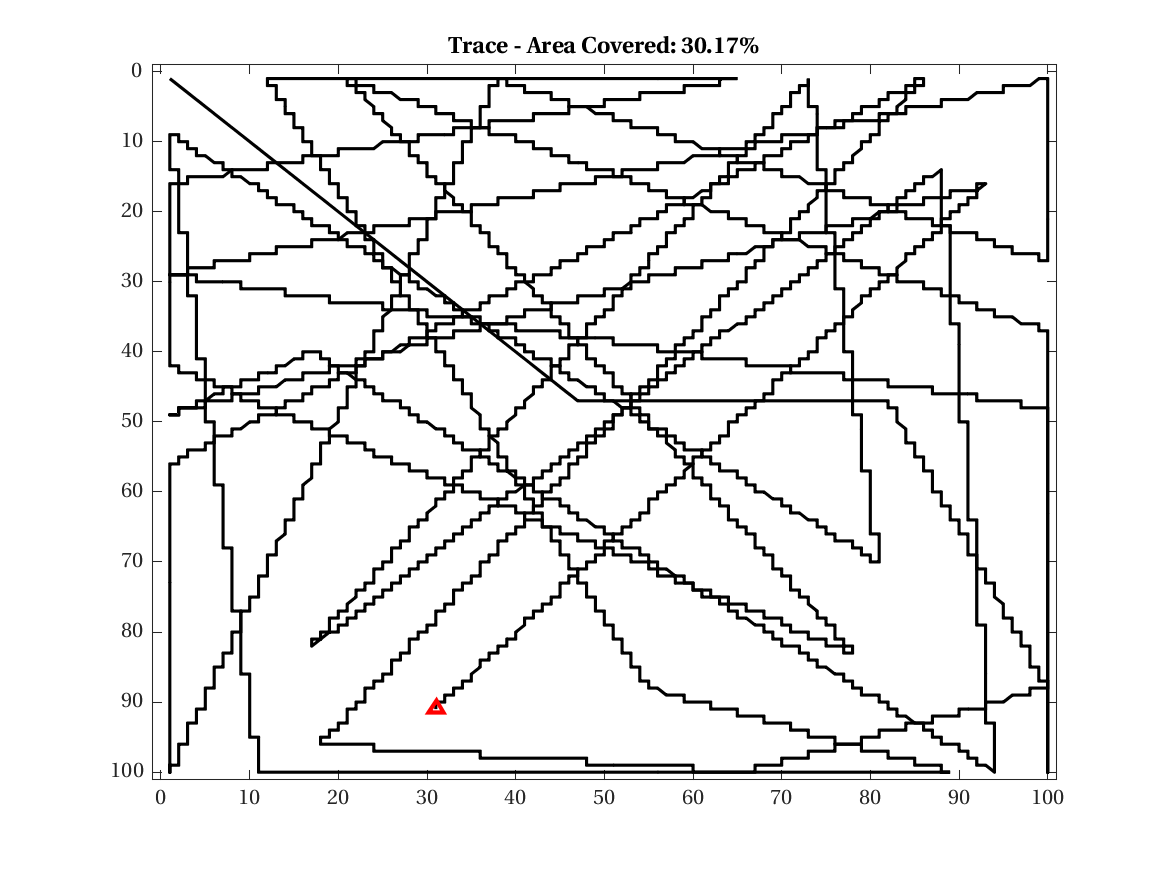
\includegraphics[width=\linewidth]{figures/hbresults/path_gr_30p_100x100_sf_50_seed_2.png}
        \captionsetup{skip=0.20\baselineskip,size=footnotesize}
        \caption{Gradient Range Ascent}
    \end{subfigure}%
    \\
    \begin{subfigure}[t]{0.3333\textwidth}
        \centering
        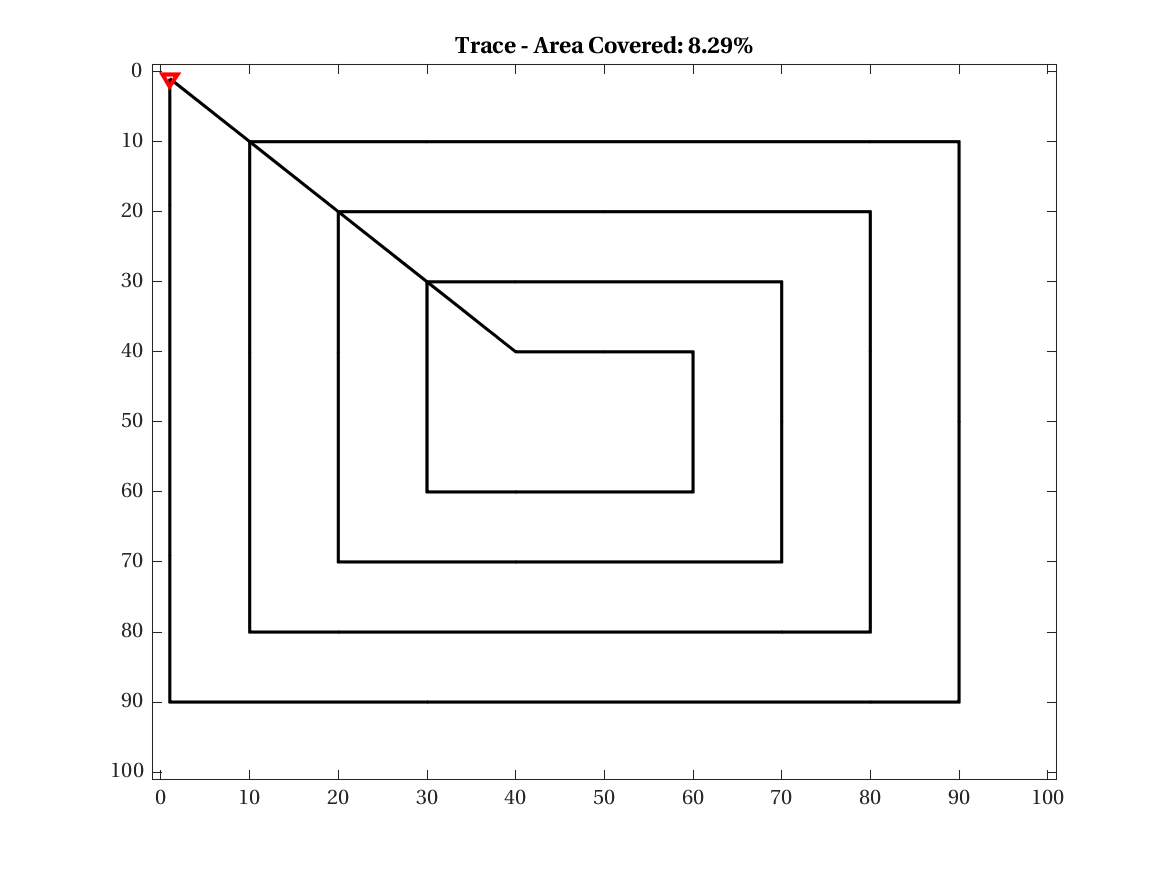
\includegraphics[width=\linewidth]{figures/hbresults/path_zz_10p_100x100_sf_50_seed_2.png}
        \captionsetup{skip=0.20\baselineskip,size=footnotesize}
        \caption{$ZZ_{10}$}
    \end{subfigure}%
    \begin{subfigure}[t]{0.3333\textwidth}
        \centering
        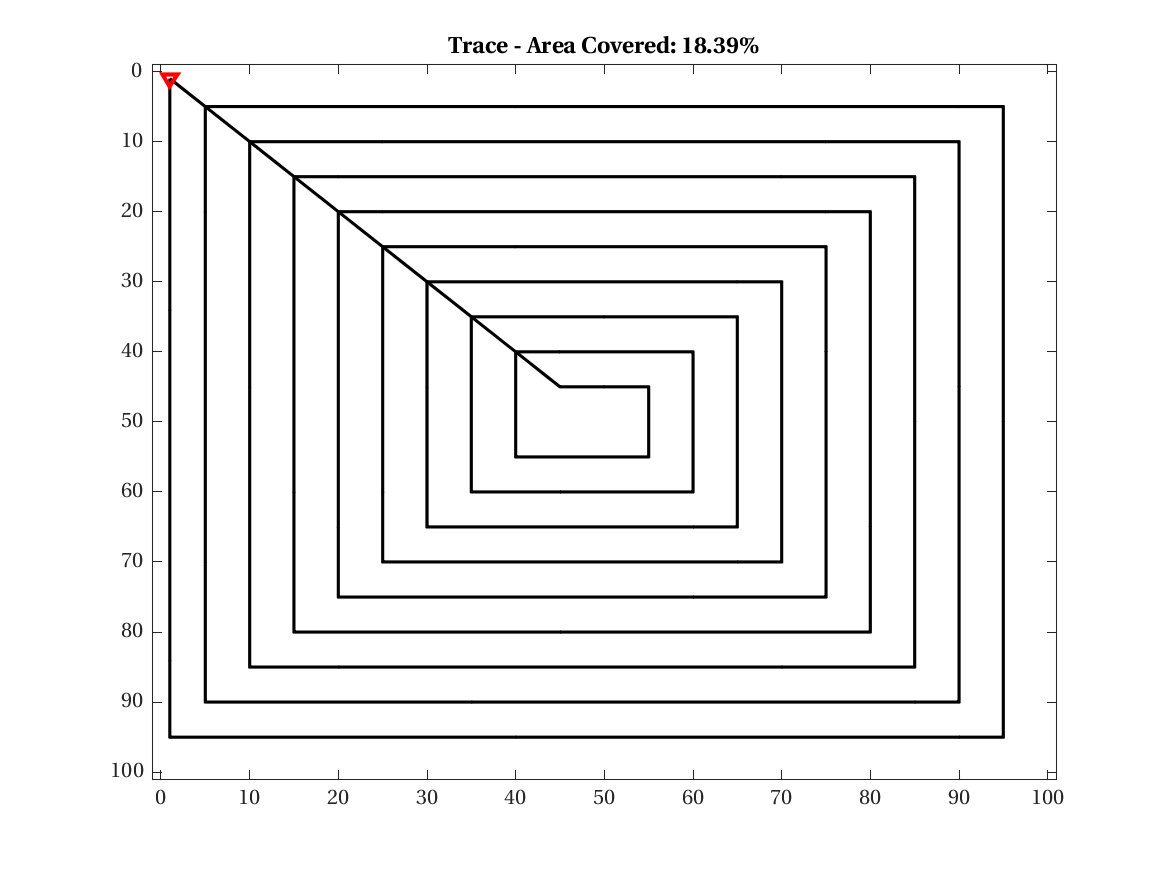
\includegraphics[width=\linewidth]{figures/hbresults/path_zz_20p_100x100_sf_50_seed_2.png}
        \captionsetup{skip=0.20\baselineskip,size=footnotesize}
        \caption{$ZZ_{20}$}
    \end{subfigure}%
    \begin{subfigure}[t]{0.3333\textwidth}
        \centering
        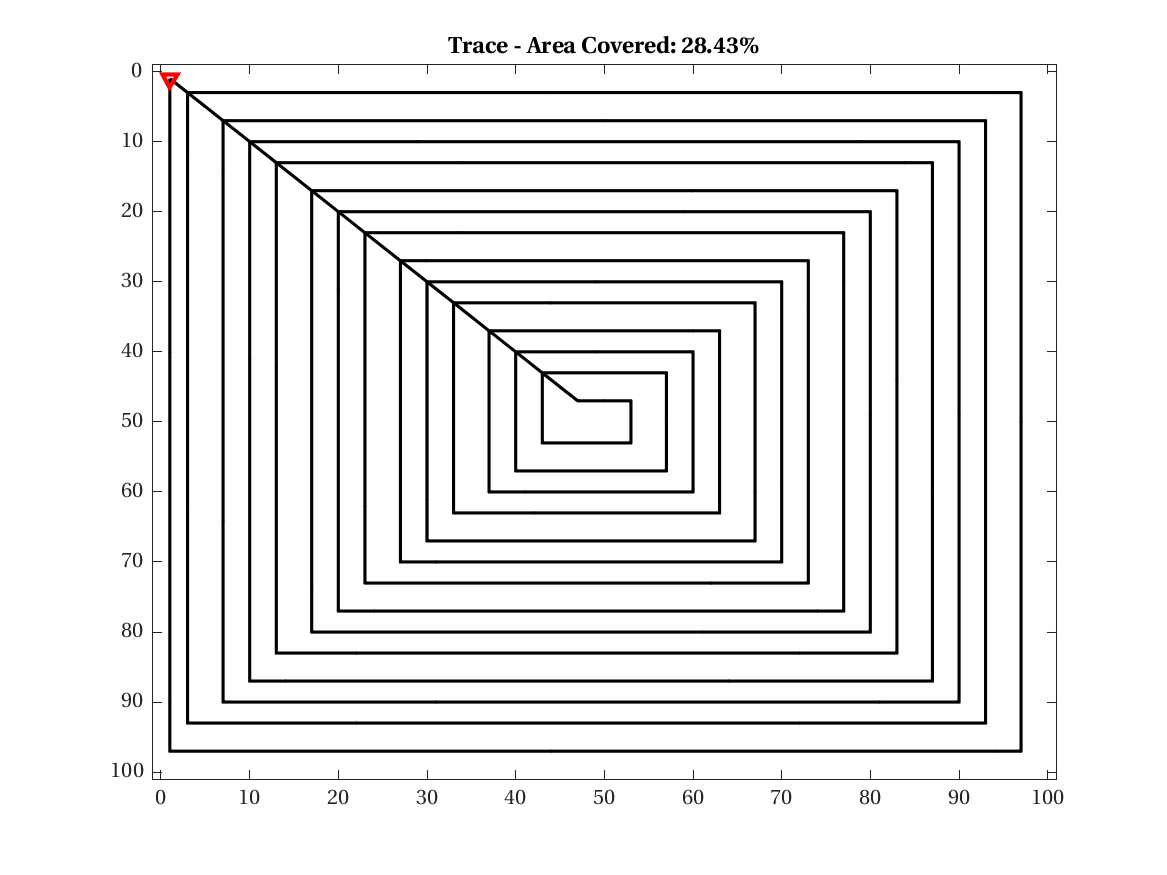
\includegraphics[width=\linewidth]{figures/hbresults/path_zz_30p_100x100_sf_50_seed_2.png}
        \captionsetup{skip=0.20\baselineskip,size=footnotesize}
        \caption{$ZZ_{30}$}
    \end{subfigure}%
    \captionsetup{skip=0.20\baselineskip}
    \caption{Exploration of a field of size $100 \times 100$, $\sigma_{field} = \frac{w}{2} = 50$, random seed 2.}
    \label{fig:sf50}
\end{figure}

\begin{figure}[htb!]
    \centering
    \begin{subfigure}[t]{0.75\textwidth}
        \centering
        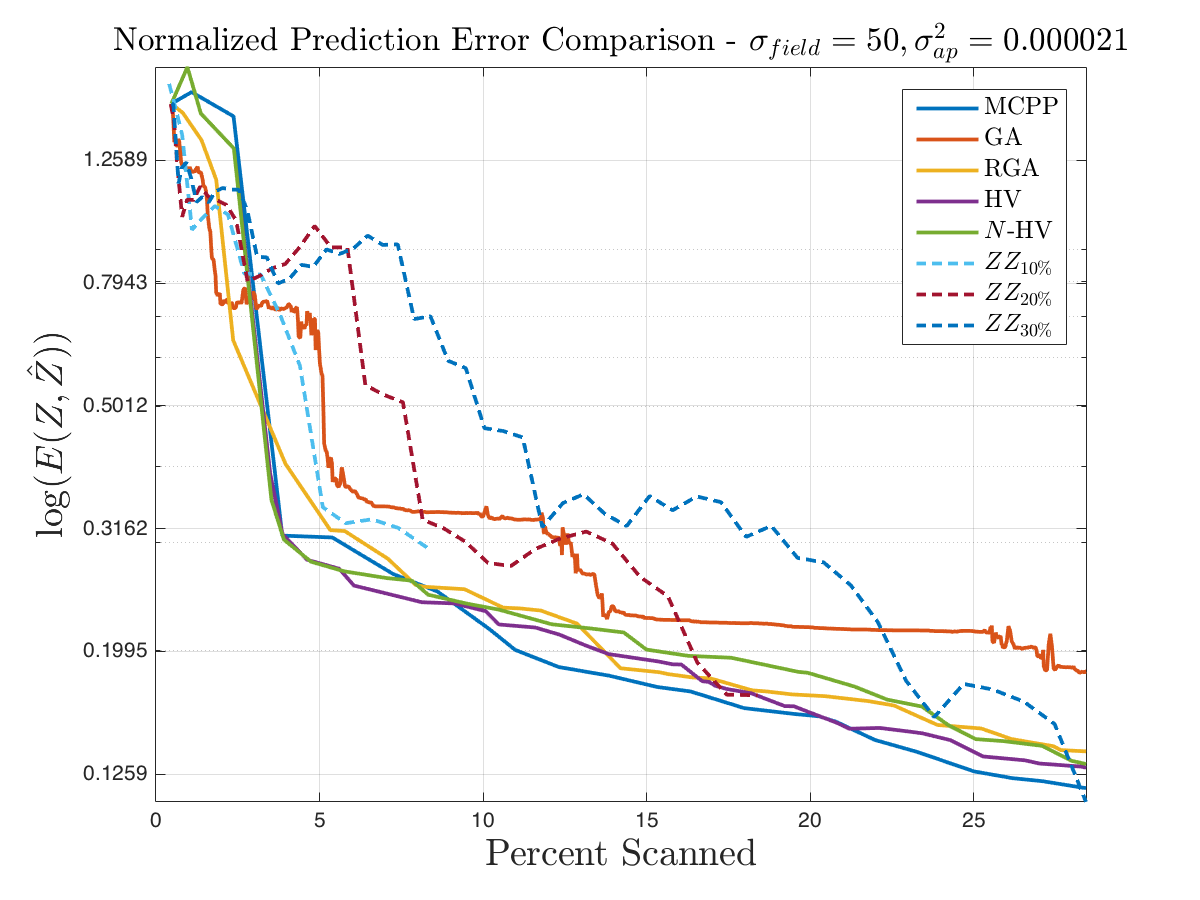
\includegraphics[width=\linewidth]{figures/results/normalized_errors_30p_100x100_sf_50_seed_2_app_50.png}
        \captionsetup{skip=0.20\baselineskip,size=footnotesize}
        \caption{Normalized prediction errors for each method.}
    \end{subfigure}%
    \\
    \begin{subfigure}[t]{0.75\textwidth}
        \centering
        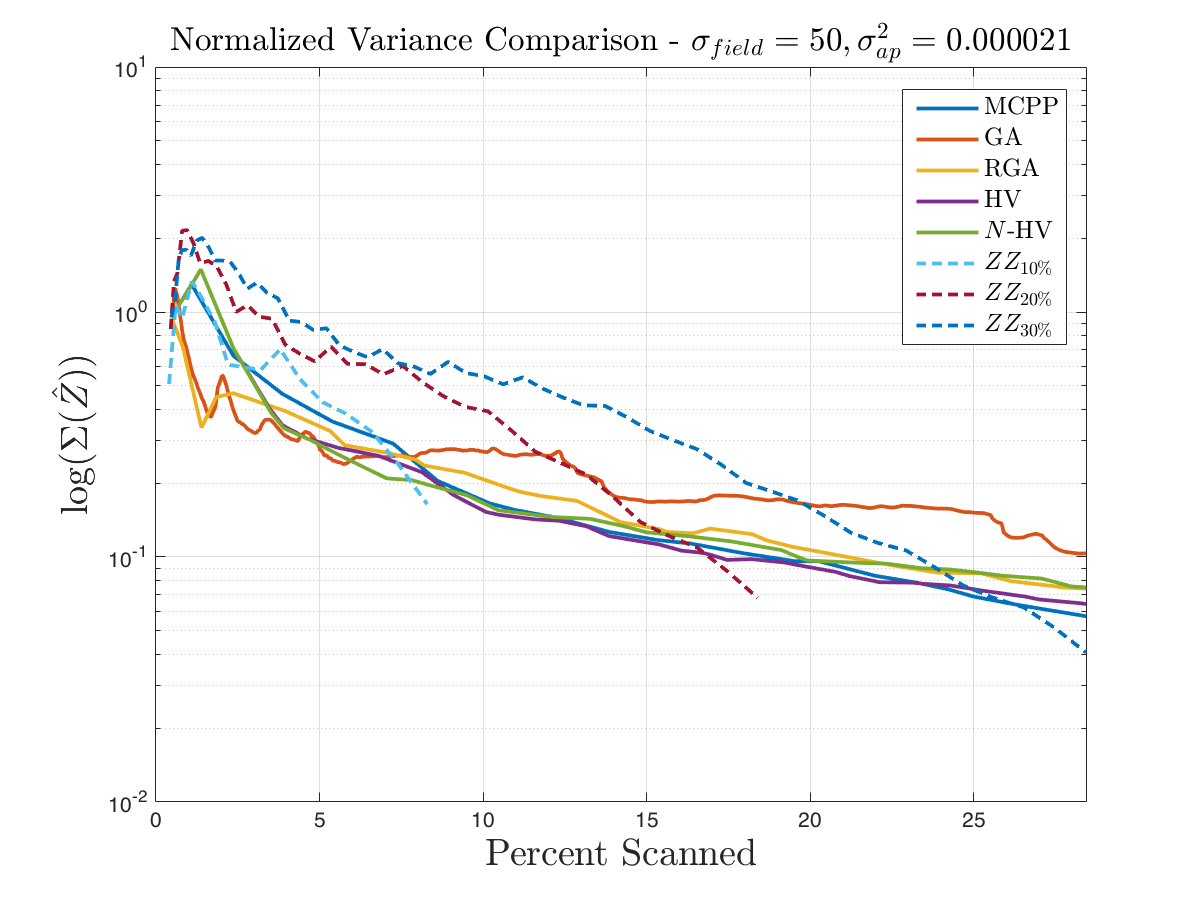
\includegraphics[width=\linewidth]{figures/results/normalized_variances_30p_100x100_sf_50_seed_2_app_50.png}
        \captionsetup{skip=0.20\baselineskip,size=footnotesize}
        \caption{Normalized prediction variances for each method.}
    \end{subfigure}%
    \captionsetup{skip=0.20\baselineskip}
    \caption{Prediction error and variances for an exploration of a field of size $100 \times 100$, $\sigma_{field} = 50$, random seed 2.}
    \label{fig:errvar50}
\end{figure}

\FloatBarrier
\clearpage

\section{Low Spatial Autocorrelation Results}
The methods will be compared on target fields generated with an autocorrelation factor, $\sigma_{field}$, equal to one. A Gaussian filter $G(x,y,1)$ (Equation \ref{eq:gauss_filt}), is convolved with all points on the field.

\begin{figure}[htb!]
    \centering
    \begin{subfigure}[t]{0.3333\textwidth}
        \centering
        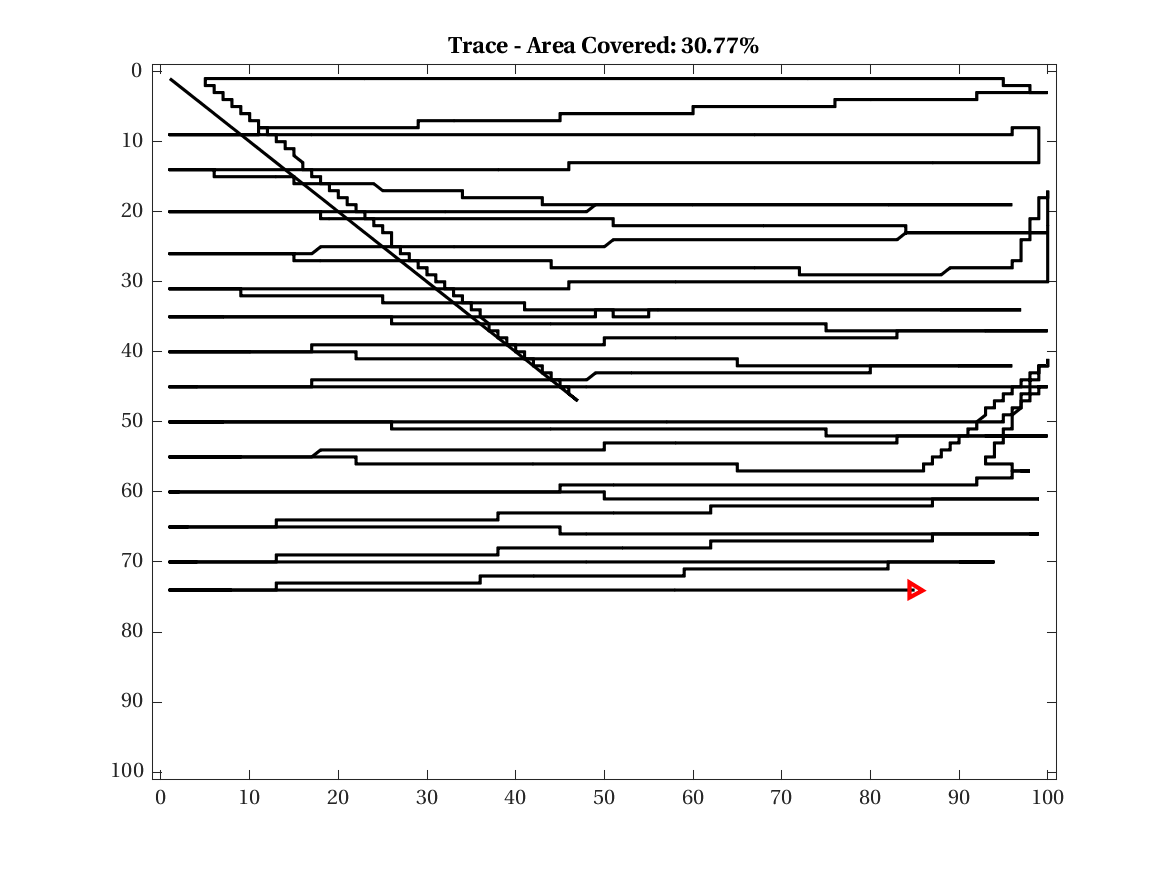
\includegraphics[width=\linewidth]{figures/hbresults/path_nhv_30p_100x100_sf_1_seed_2.png}
        \captionsetup{skip=0.20\baselineskip,size=footnotesize}
        \caption{Highest Variance}
    \end{subfigure}%
    \begin{subfigure}[t]{0.3333\textwidth}
        \centering
        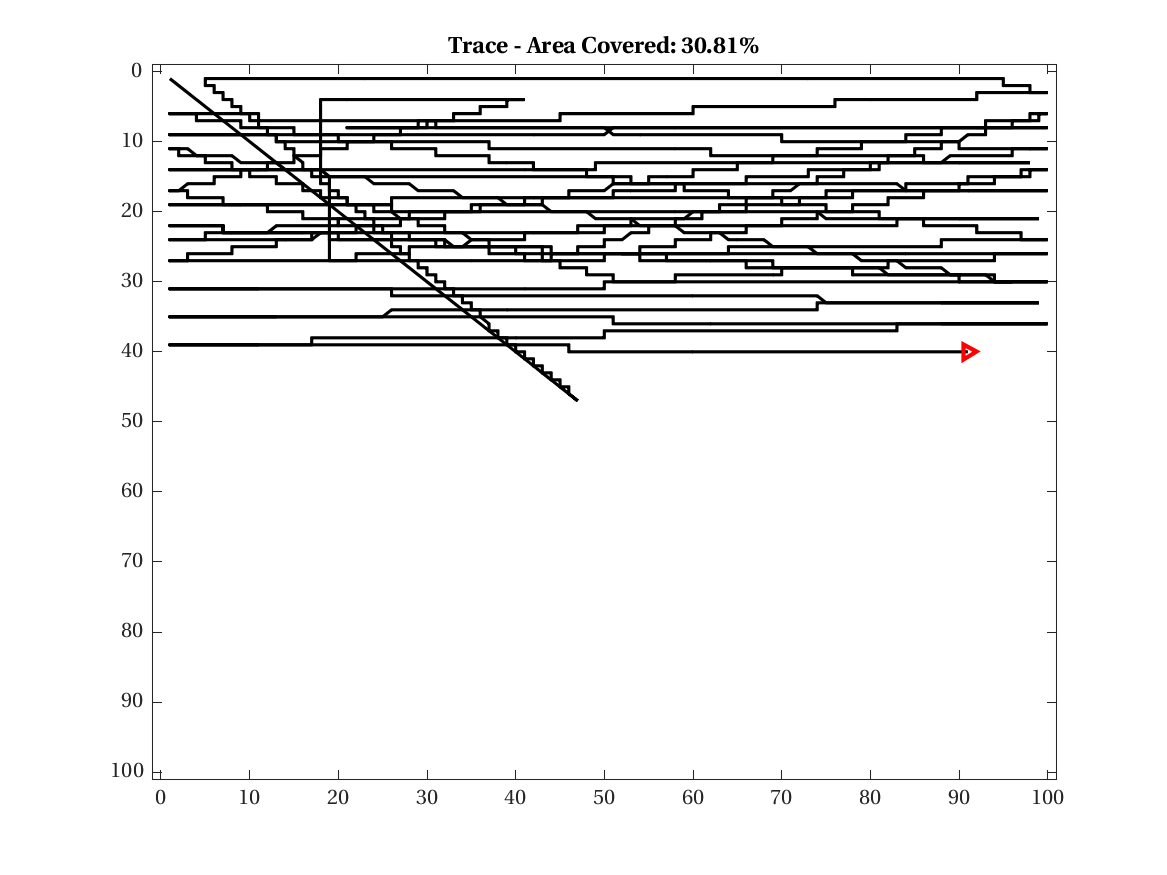
\includegraphics[width=\linewidth]{figures/hbresults/path_nnhv_30p_100x100_sf_1_seed_2.png}
        \captionsetup{skip=0.20\baselineskip,size=footnotesize}
        \caption{$N$ Highest Variance}
    \end{subfigure}%
    \begin{subfigure}[t]{0.3333\textwidth}
        \centering
        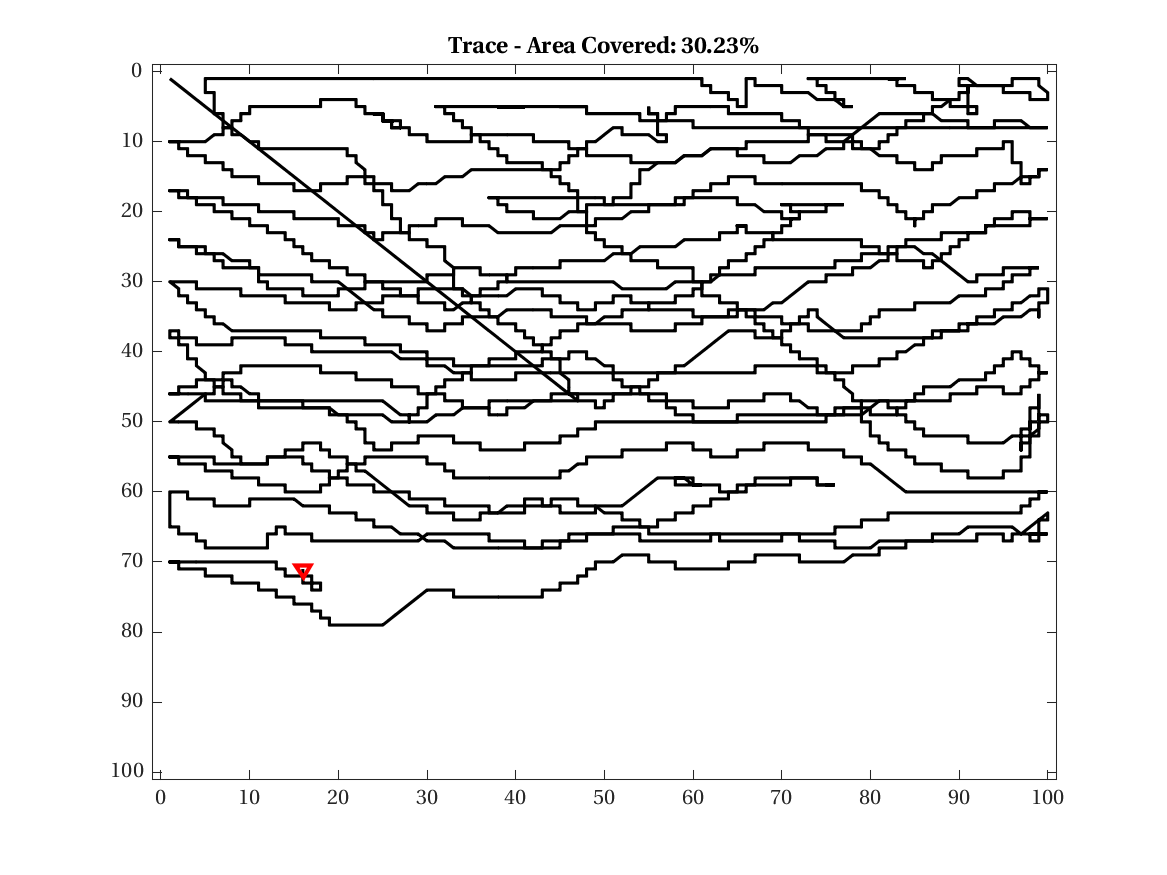
\includegraphics[width=\linewidth]{figures/hbresults/path_mc_30p_100x100_sf_1_seed_2.png}
        \captionsetup{skip=0.20\baselineskip,size=footnotesize}
        \caption{Monte Carlo}
    \end{subfigure}%
    \\
    \begin{subfigure}[t]{0.3333\textwidth}
        \centering
        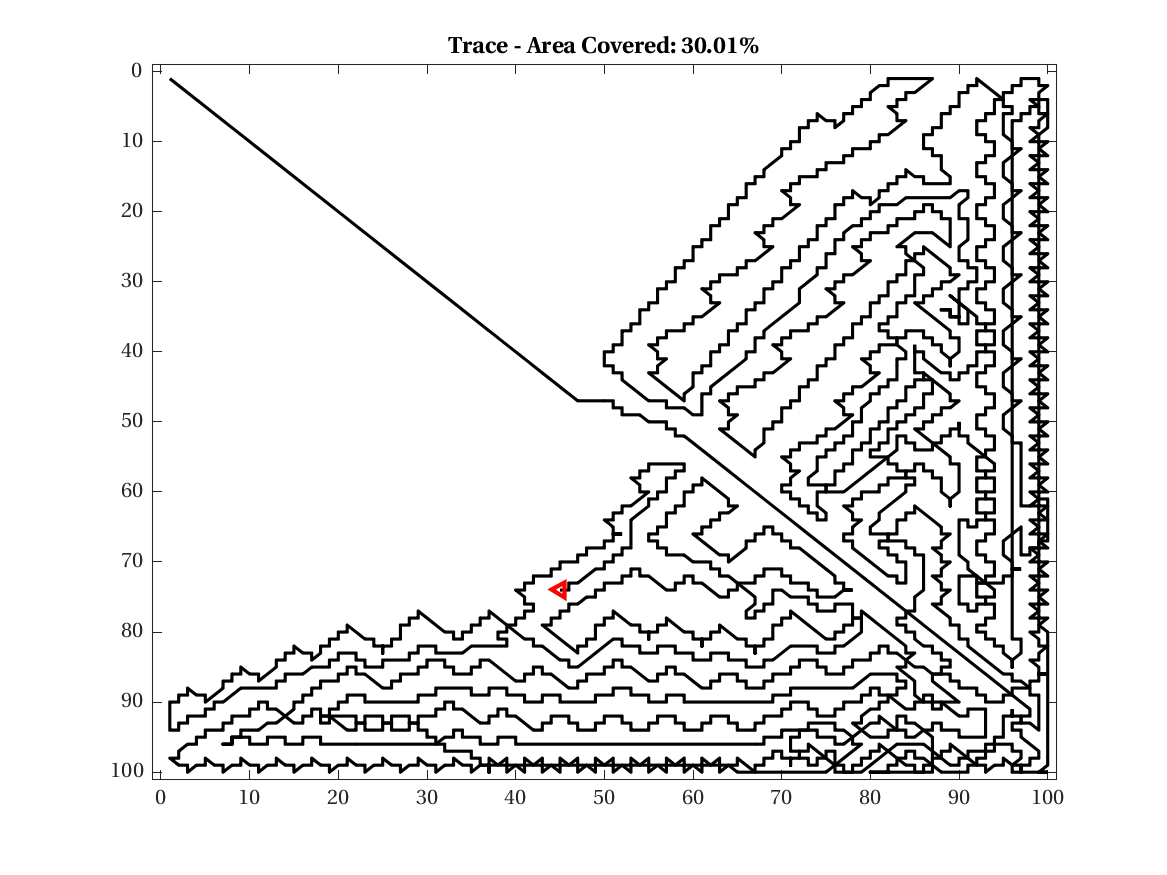
\includegraphics[width=\linewidth]{figures/hbresults/path_gradient_30p_100x100_sf_1_seed_2.png}
        \captionsetup{skip=0.20\baselineskip,size=footnotesize}
        \caption{Gradient Ascent}
    \end{subfigure}%
    \begin{subfigure}[t]{0.3333\textwidth}
        \centering
        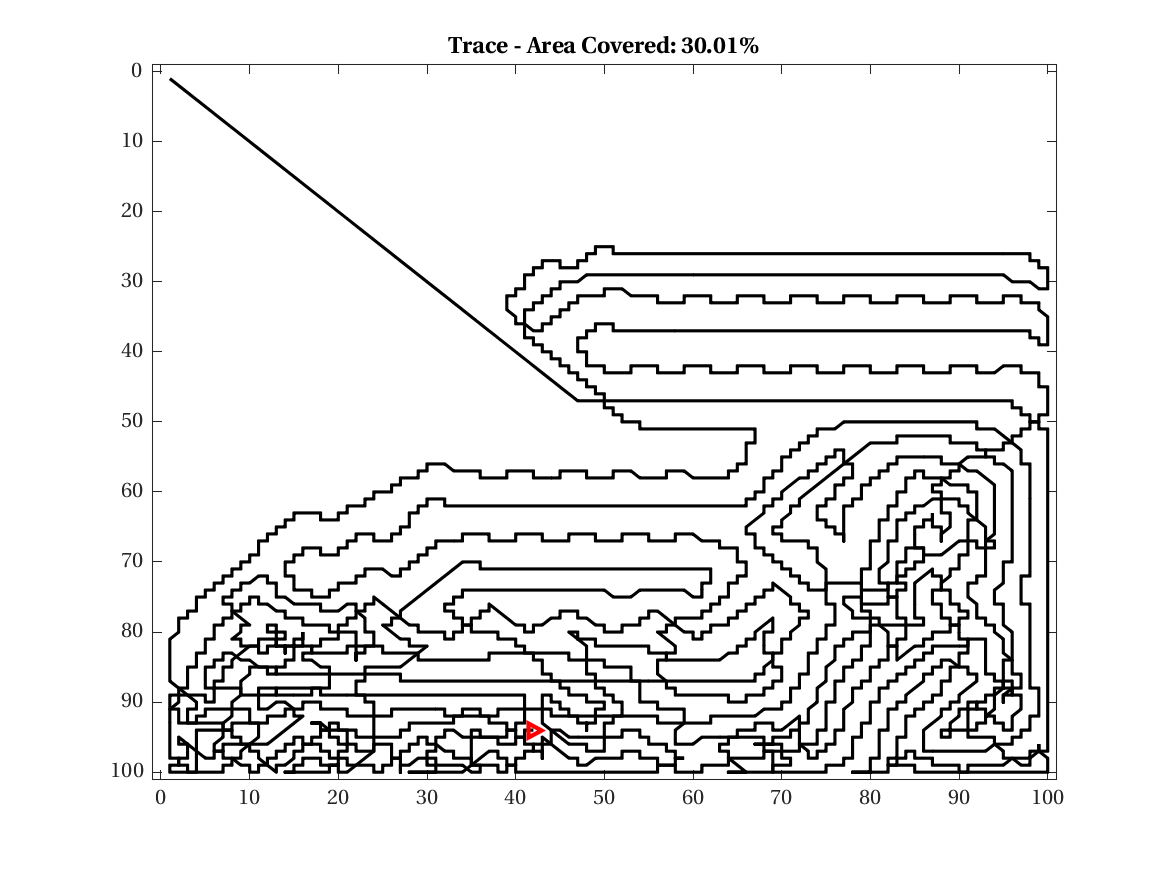
\includegraphics[width=\linewidth]{figures/hbresults/path_gr_30p_100x100_sf_1_seed_2.png}
        \captionsetup{skip=0.20\baselineskip,size=footnotesize}
        \caption{Gradient Range Ascent}
    \end{subfigure}%
    \\
    \begin{subfigure}[t]{0.3333\textwidth}
        \centering
        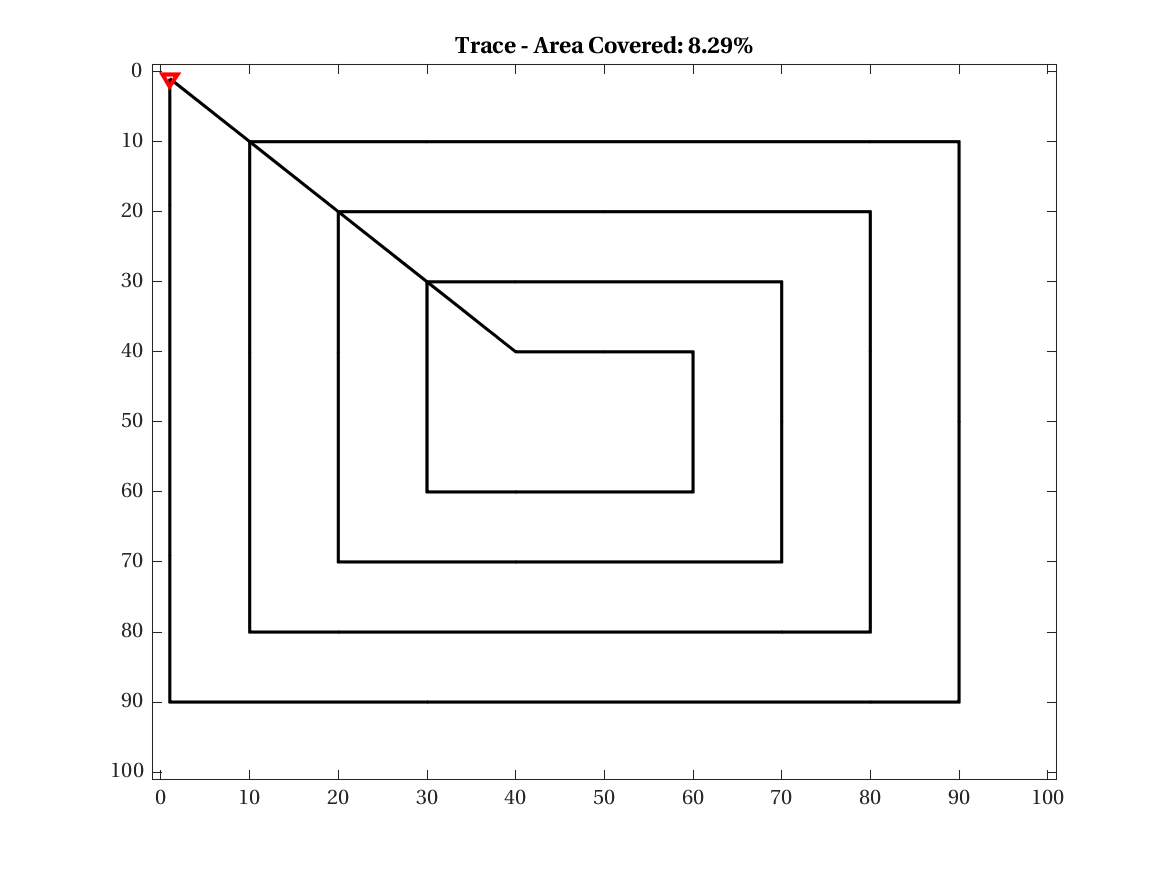
\includegraphics[width=\linewidth]{figures/hbresults/path_zz_10p_100x100_sf_1_seed_2.png}
        \captionsetup{skip=0.20\baselineskip,size=footnotesize}
        \caption{$ZZ_{10}$}
    \end{subfigure}%
    \begin{subfigure}[t]{0.3333\textwidth}
        \centering
        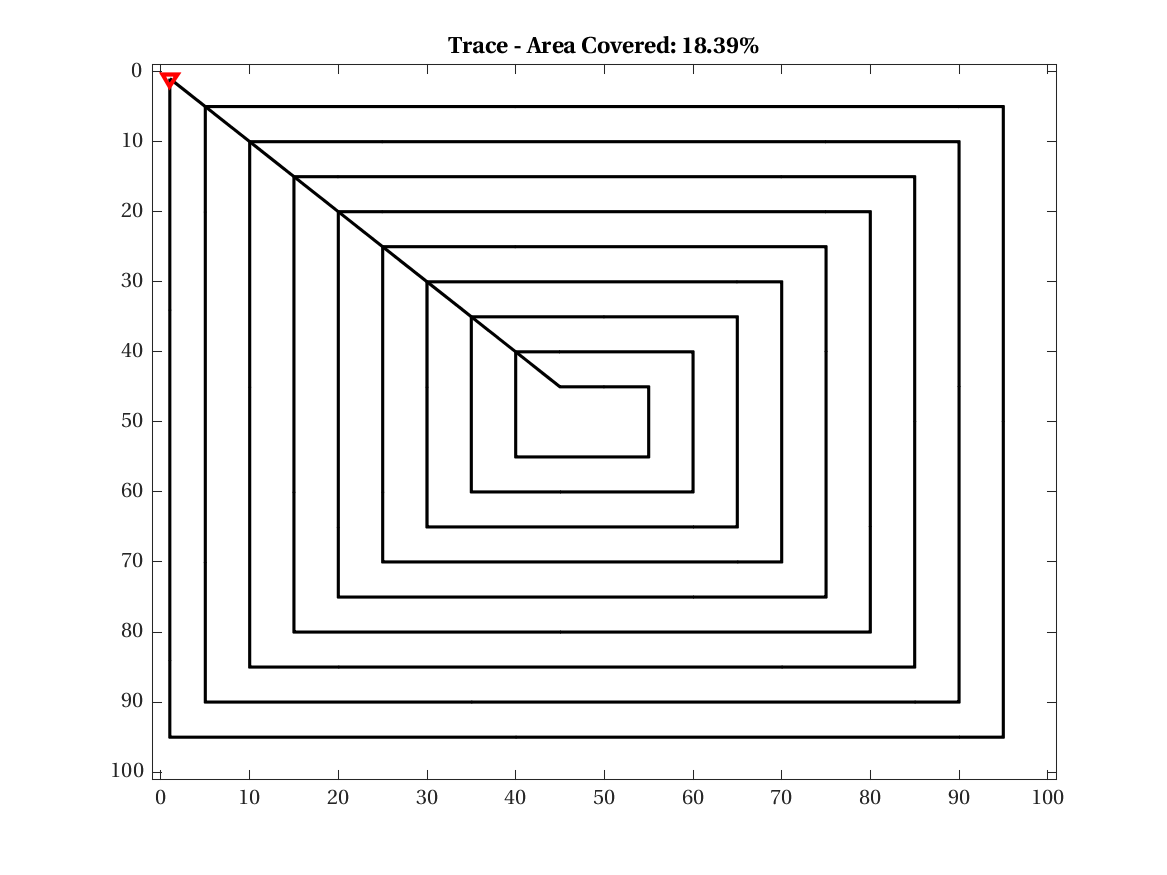
\includegraphics[width=\linewidth]{figures/hbresults/path_zz_20p_100x100_sf_1_seed_2.png}
        \captionsetup{skip=0.20\baselineskip,size=footnotesize}
        \caption{$ZZ_{20}$}
    \end{subfigure}%
    \begin{subfigure}[t]{0.3333\textwidth}
        \centering
        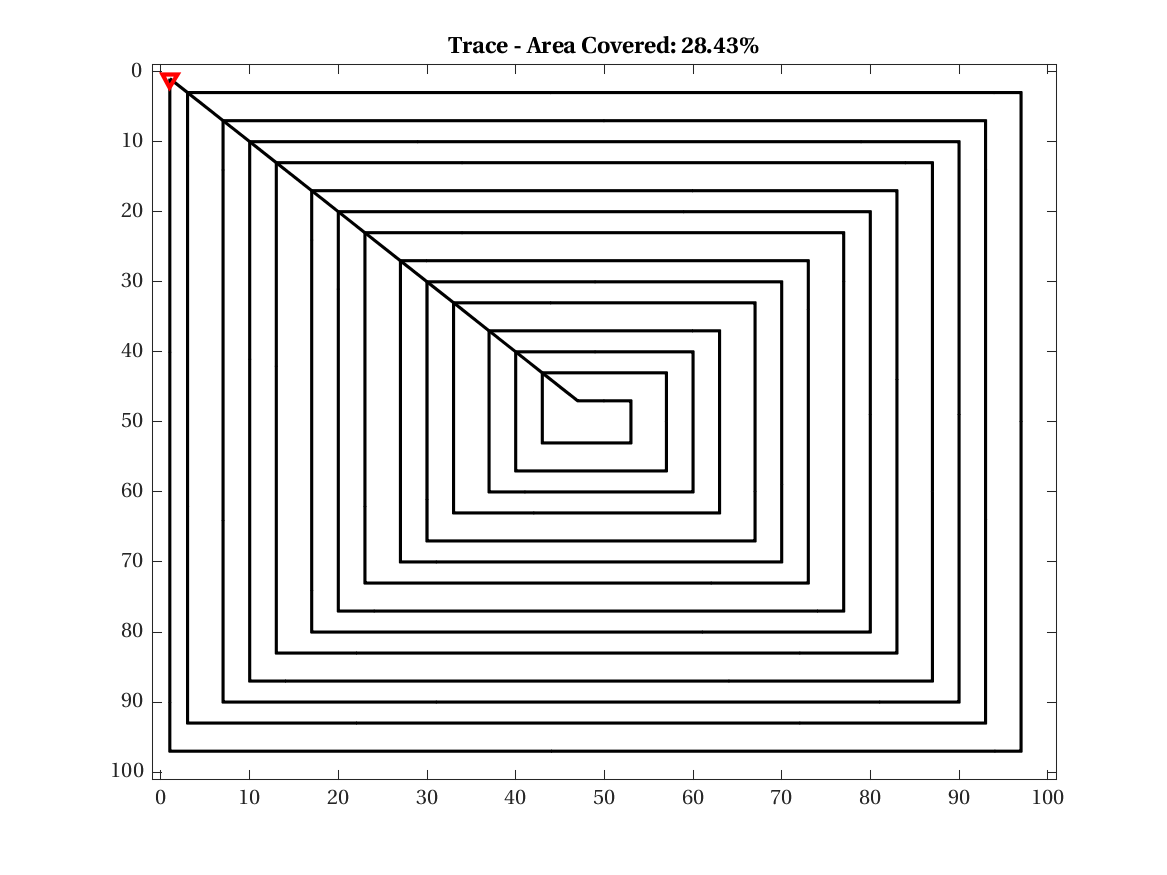
\includegraphics[width=\linewidth]{figures/hbresults/path_zz_30p_100x100_sf_1_seed_2.png}
        \captionsetup{skip=0.20\baselineskip,size=footnotesize}
        \caption{$ZZ_{30}$}
    \end{subfigure}%
    \captionsetup{skip=0.20\baselineskip}
    \caption{Exploration of a field of size $100 \times 100$, $\sigma_{field} = 1$, random seed 2.}
    \label{fig:sf1}
\end{figure}

\begin{figure}[htb!]
    \centering
    \begin{subfigure}[t]{0.75\textwidth}
        \centering
        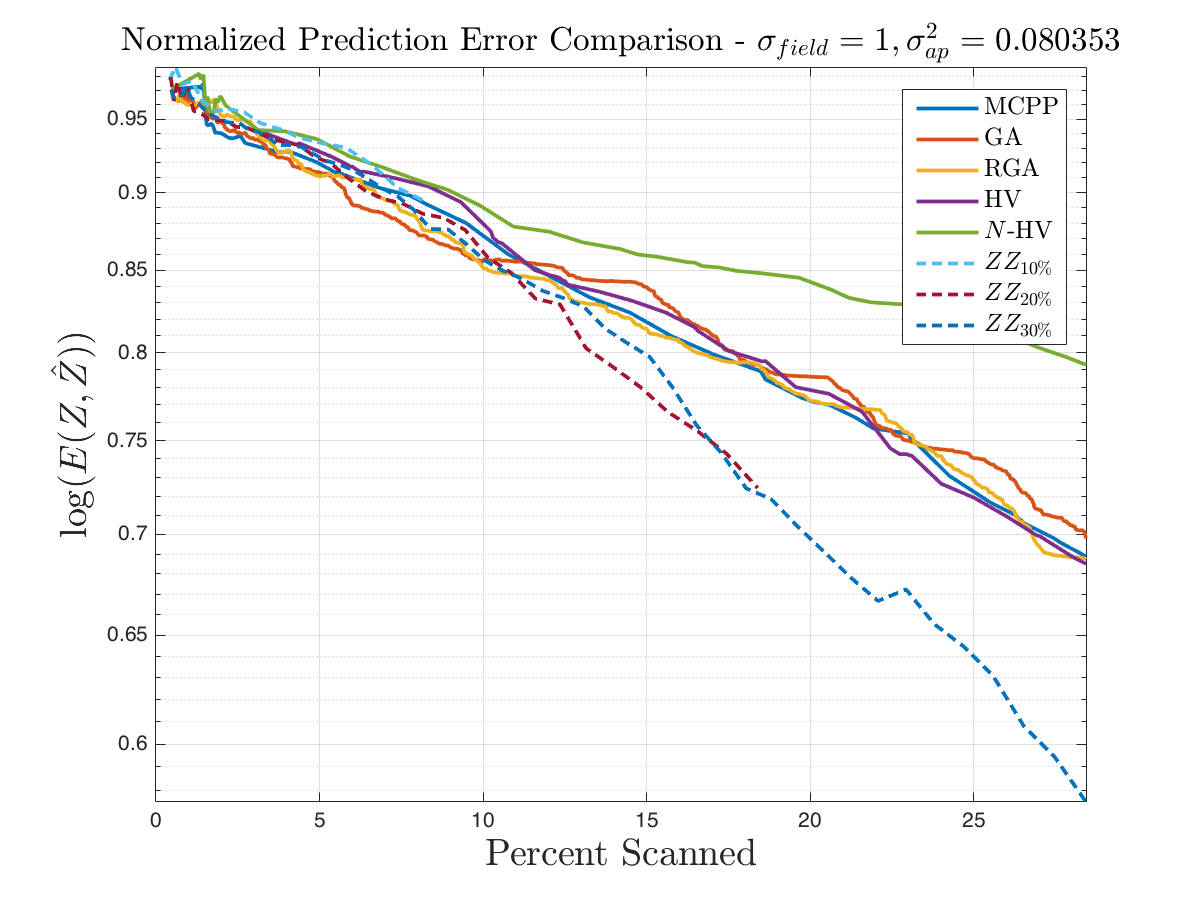
\includegraphics[width=\linewidth]{figures/results/normalized_errors_30p_100x100_sf_1_seed_2_app_50.png}
        \captionsetup{skip=0.20\baselineskip,size=footnotesize}
        \caption{Normalized prediction errors for each method.}
    \end{subfigure}%
    \\
    \begin{subfigure}[t]{0.75\textwidth}
        \centering
        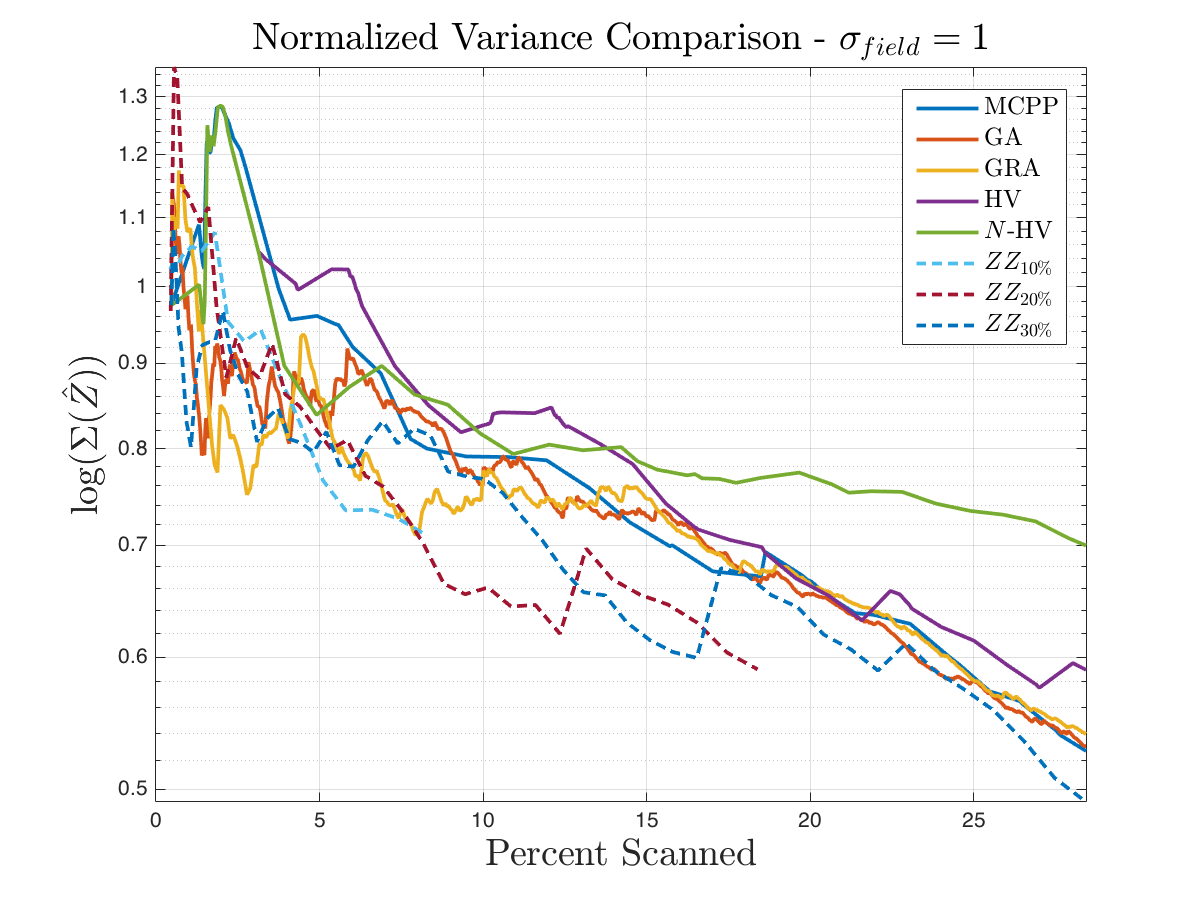
\includegraphics[width=\linewidth]{figures/results/normalized_variances_30p_100x100_sf_1_seed_2_app_50.png}
        \captionsetup{skip=0.20\baselineskip,size=footnotesize}
        \caption{Normalized prediction variances for each method.}
    \end{subfigure}%
    \captionsetup{skip=0.20\baselineskip}
    \caption{Prediction error and variances for an exploration of a field of size $100 \times 100$, $\sigma_{field} = 1$, random seed 2.}
    \label{fig:errvar1}
\end{figure}

\FloatBarrier
\clearpage

\section{Comparing The Methods}
While all of the path planners reduce Kriging prediction variance and errors in Section \ref{sec:s2_nbvcomp} and Appendix \ref{sec:s3_nbvcomp}, the Greedy Next-Best-View method finishes the $40\%$ field scan with the highest prediction error and highest prediction variance. The Range Gradient Ascent, Monte Carlo Path Planner, and Gradient Ascent methods performed the best out of the other methods. This is likely due to the Greedy NBV method's inability to scan points of high variance directly as discussed in Section \ref{sec:discuss}. The benefits in Greedy NBV lie in its computational simplicity when compared to the trajectory calculating methods like MCPP and $N$-HV. When comparing computational complexity, the HV method selects a point less often than the Greedy NBV method, and when the point is selected, is identical. The GA and RGA methods theoretically run in the same runtime in terms of selection ($\Theta(hw)$). From the simulated results, HV, GA, and RGA would generate better quality mapping over Greedy NBV for a given field with these spatial autocorrelation factors, and would require the same computational ability. 

All of the path planning methods reduce prediction variance as they scan more area, for all runs of varying spatial autocorrelation, field, and random seed. The prediction errors drop proportionally to the prediction variance lost over area scanned. The hypothesis that purposefully minimizing Kriging prediction variance in turn reduces prediction error (stated in Section \ref{sec:fielduncert}) has been demonstrated to be true for the results show in this chapter and in Appendix \ref{app:add_results}. 

The results show that a field becomes more predictable when it has a larger spatial autocorrelation factor. This is due to the fact that the Kriging method predicts more accurately if more spatial traits of the field are known and ``obvious'' to the predictor. When the field is highly predictable (higher values of $\sigma_{field}$), a variance suppressing path planner, like the planners introduced in this thesis, perform better than preplanned paths which do not attempt to directly reduce prediction variance. When comparing the Monte Carlo Path Planner against the zig-zag method for varying autocorrelation factors and varying random seeds (Figures \ref{fig:multaccomp_s2} and \ref{fig:multaccomp_s3}), the Monte Carlo path planner reduces prediction error and prediction variance to a higher degree for most of the scanning processes. The lower prediction errors associated with MCPP come at the cost of calculating the expected return on a larger number of candidate trajectories ($NM_{mc}$) when compared to any of the other methods. 

When the autocorrelation factor of the field is low, the preplanned method performs better at reducing prediction error. Unlike the exploration of fields with higher factors of spatial autocorrelation, both the MCPP and $N$-HV methods performed poorly for fields with low autocorrelation. This is likely due to feeding back Kriging predictions in the path planning process from poorly predicted points. Furthermore, points near by the exploration vehicle have equally high variances to far away points. The other variance suppressing path planners similarly performed poorly for fields with lower autocorrelations, as there is no guarantee that a field with a low autocorrelation factor will be evenly explored with one of the variance suppressing methods introduced. The differences in the paths taken show that the zig-zag method uniformly scans the field, while the other methods only sample more isolated regions on the field as they become ``stuck'' scanning in nearby low variance regions until they meet their scan limits. This implies that for lower spatial autocorrelation in a field, a more evenly distributed sampling regime over the field might reduce prediction error and variance more than directly focusing on reducing prediction variance alone.

The spatial autocorrelation factor of a target field was shown to be directly proportional to the ability of the non-preplanned planners to explore the field. The proportionality was shown to be true with little variability among different random seeds.

\begin{figure}[htb!]
    \centering
    \begin{subfigure}[t]{0.75\textwidth}
        \centering
        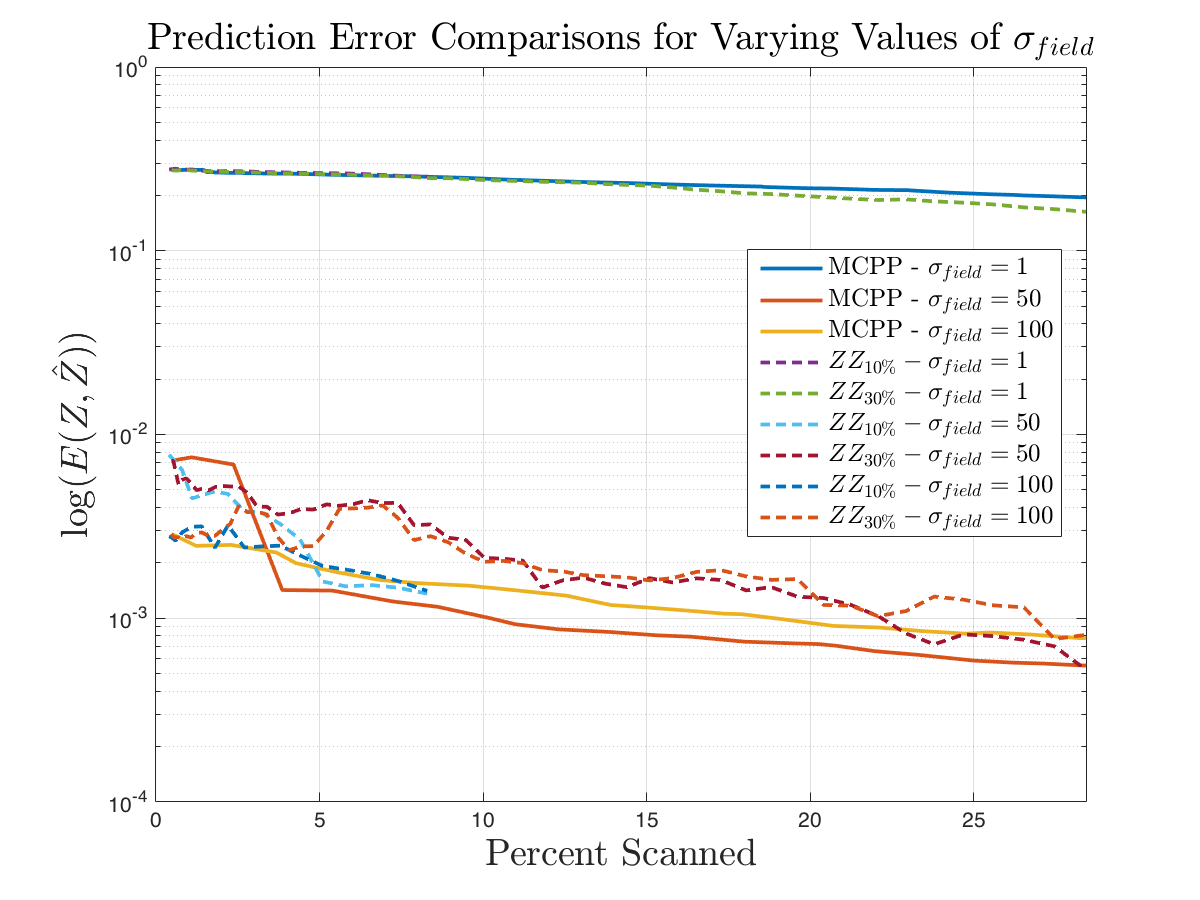
\includegraphics[width=\linewidth]{figures/results/errors_30p_100x100_sf_all_seed_2_app_0.png}
        \captionsetup{skip=0.20\baselineskip,size=footnotesize}
        \caption{Normalized prediction errors for MCPP and ZZ for $\sigma_{field} = \{1, 50, 100\}$.}
    \end{subfigure}%
    \\
    \begin{subfigure}[t]{0.75\textwidth}
        \centering
        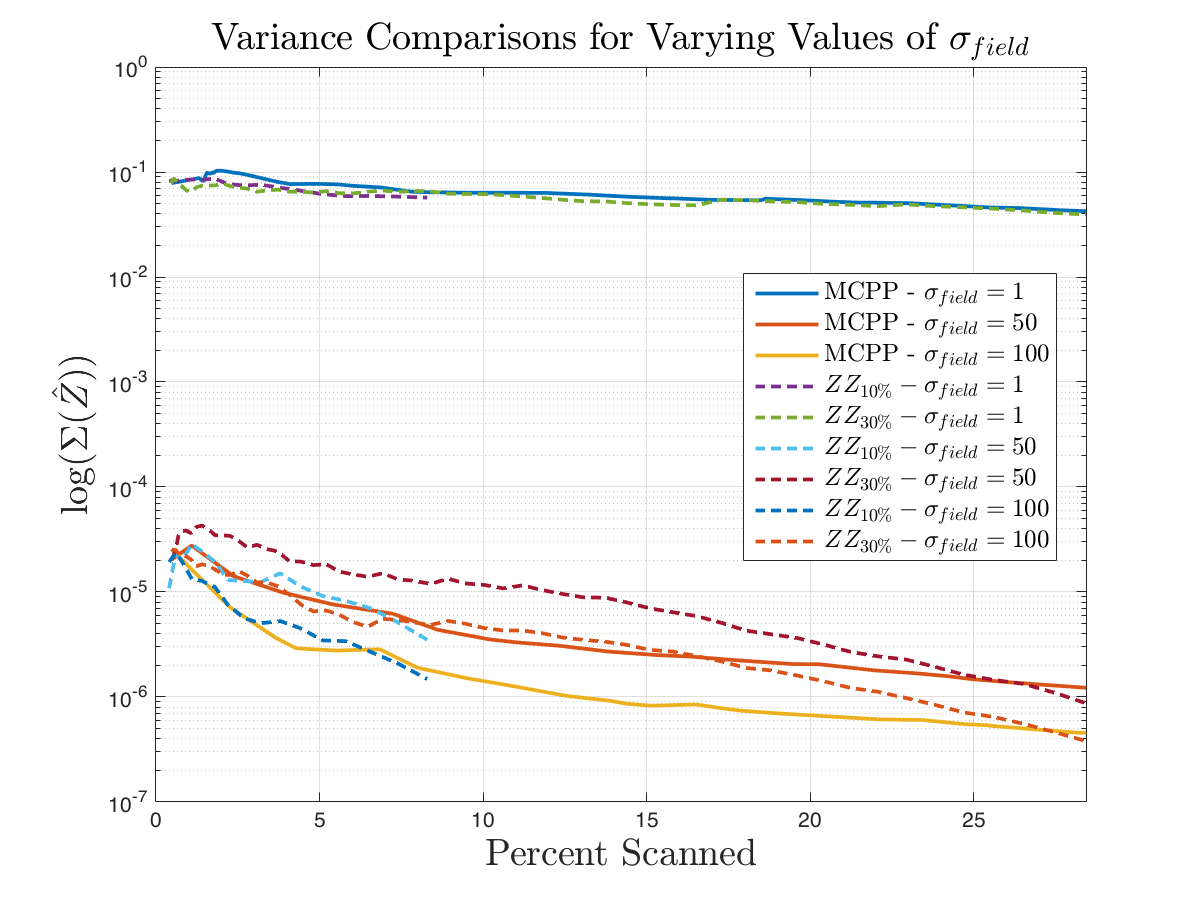
\includegraphics[width=\linewidth]{figures/results/variances_30p_100x100_sf_all_seed_2_app_0.png}
        \captionsetup{skip=0.20\baselineskip,size=footnotesize}
        \caption{Normalized prediction variances for MCPP and ZZ for $\sigma_{field} = \{1, 50, 100\}$.}
    \end{subfigure}%
    \ssp
    \captionsetup{skip=0.20\baselineskip}
    \caption{Prediction error and variances for an exploration of $3$ different fields of size $100 \times 100$ for autocorrelation factors of $\sigma_{field} = 1$, $\sigma_{field} = 50$, $\sigma_{field} = 100$ respectively. Random seed 2.}
    \label{fig:multaccomp_s2}
\end{figure}
\begin{figure}[htb!]
    \centering
    \begin{subfigure}[t]{0.75\textwidth}
        \centering
        \includegraphics[width=\linewidth]{figures/results/errors_30p_100x100_sf_all_seed_3_app_0.png}
        \captionsetup{skip=0.20\baselineskip,size=footnotesize}
        \caption{Normalized prediction errors for MCPP and ZZ for $\sigma_{field} = \{1, 50, 100\}$.}
    \end{subfigure}%
    \\
    \begin{subfigure}[t]{0.75\textwidth}
        \centering
        \includegraphics[width=\linewidth]{figures/results/variances_30p_100x100_sf_all_seed_3_app_0.png}
        \captionsetup{skip=0.20\baselineskip,size=footnotesize}
        \caption{Normalized prediction variances for MCPP and ZZ for $\sigma_{field} = \{1, 50, 100\}$.}
    \end{subfigure}%
    \ssp
    \captionsetup{skip=0.20\baselineskip}
    \caption{Prediction error and variances for an exploration of $3$ different fields of size $100 \times 100$ for autocorrelation factors of $\sigma_{field} = 1$, $\sigma_{field} = 50$, $\sigma_{field} = 100$ respectively. Random seed 3.}
    \label{fig:multaccomp_s3}
\end{figure}
\FloatBarrier
% \clearpage

When compared to the planners introduced, along with the zig-zag method, the Gradient Ascent planner performs the worst in terms of reducing prediction error and variance for size $100 \times 100$ fields, even with higher autocorrelation factors. This is likely due to the planner limiting its movement to the area directly around it. The planner does not focus on reducing overall field uncertainty globally, but more specifically in the local vicinity of the field, similarly to the Greedy NBV method. The Range Gradient Ascent and Highest Variance planners reduce prediction error more effectively over the standard Gradient Ascent method likely because of their ability to explore and minimize prediction variances more globally. RGA, HV, and $N$-HV explore the field by purposefully targeting farther points that are likely to have higher prediction uncertainty by considering points at the edge and outside of the range of autocorrelation on the field. Gradient Ascent was an attempt at hill climbing the variance field. It did not perform well for larger fields because the hills and valleys of the variance field radically change at each decision point in the exploration process. Climbing to the point of highest nearest variance in an effort to maximize variance loss, in an effort to reduce overall field variance, relies on the assumption that the variance field is static. Variance fields were shown to be dynamic, as a function of spatial autocorrelation, as more samples are taken in an exploration process.

\section{Real World Considerations}
For an exploration vehicle implementing one or more of the introduced planners on a real system, the computational load required to calculate the Kriging predictions and variances may be a limiting factor. As target field sizes increase, the computational load required to invert large poorly conditioned matrices may be unrealistic or infeasible. In order to perform a real life exploration, the number of vesicles on the target field must be tuned to meet the requirements (memory and processing power) of the exploration system and minimum exploration specifications. 

The initial waypoint in a real exploration mission can be set to any desired point, and is not limited to the point selected in the simulations presented. A consideration to make with regards to setting an initial waypoint is that the variance suppressing path planners require an initial set of samples on the field to make an initial. The first waypoint selected should be at a large enough distance from the starting position so that the planners have enough samples to make a decent initial decision. 

Since the variance suppressing planners do not perform well in fields with low levels of spatial autocorrelation, dynamically switching to a preplanned trajectory, like the zig-zag method, might be a useful tactic for exploring a field. The autocorrelation range of the field learned after computing the initial variogram model for the target field can be used to determine whether a preplanned trajectory may yield better results.
